% ****** Start of file apssamp.tex ******
%
%   This file is part of the APS files in the REVTeX 4.1 distribution.
%   Version 4.1r of REVTeX, August 2010
%
%   Copyright (c) 2009, 2010 The American Physical Society.
%
%   See the REVTeX 4 README file for restrictions and more information.
%
% TeX'ing this file requires that you have AMS-LaTeX 2.0 installed
% as well as the rest of the prerequisites for REVTeX 4.1
%
% See the REVTeX 4 README file
% It also requires running BibTeX. The commands are as follows:
%
%  1)  latex apssamp.tex
%  2)  bibtex apssamp
%  3)  latex apssamp.tex
%  4)  latex apssamp.tex
%
\documentclass[%
 reprint,
%superscriptaddress,
%groupedaddress,
%unsortedaddress,
%runinaddress,
%frontmatterverbose, 
%preprint,
%showpacs,preprintnumbers,
%nofootinbib,
%nobibnotes,
%bibnotes,
 amsmath,amssymb,
 aps,
%pra,
%prb,
%rmp,
prstab,
%prstper,
%floatfix,
]{revtex4-1}

\usepackage{graphicx}% Include figure files
\usepackage{dcolumn}% Align table columns on decimal point
\usepackage{bm}% bold math
%\usepackage{hyperref}% add hypertext capabilities
%\usepackage[mathlines]{lineno}% Enable numbering of text and display math
%\linenumbers\relax % Commence numbering lines
\usepackage{color}
\usepackage{siunitx}
\usepackage{url}

%\usepackage[showframe,%Uncomment any one of the following lines to test 
%%scale=0.7, marginratio={1:1, 2:3}, ignoreall,% default settings
%%text={7in,10in},centering,
%%margin=1.5in,
%%total={6.5in,8.75in}, top=1.2in, left=0.9in, includefoot,
%%height=10in,a5paper,hmargin={3cm,0.8in},
%]{geometry}

\DeclareFontFamily{U}{wncy}{}
\DeclareFontShape{U}{wncy}{m}{n}{<->wncyr10}{}
\DeclareSymbolFont{mcy}{U}{wncy}{m}{n}
\DeclareMathSymbol{\Sh}{\mathord}{mcy}{"58} 

\newcommand{\q}[2]{\ensuremath{#1\ \mathrm{#2}}} % quantity with units

\begin{document}

%\title{Effects of pulsed hollow electron lens operation on the beam core in HL-LHC: \\First experimental studies and simulations.}% Force line breaks with \\
\title{Effect of resonant and random excitation on the LHC beam in the context of pulsed hollow electron lens operation.}% Force line breaks with \\
\thanks{Fermilab is operated by Fermi Research Alliance, LLC under
	Contract No.~DE-AC02-07CH11359 with the United States Department of
	Energy. This work was partially supported by the US DOE LHC
	Accelerator Research Program (LARP) and by the European FP7 HiLumi
	LHC Design Study, Grant Agreement 284404.}

\author{Miriam Fitterer}
 \email{mfittere@fnal.gov}
\author{Giulio Stancari}%
\author{Alexander Valishev}%
\affiliation{Fermi National Accelerator Laboratory, Batavia, Illinois, USA
% This line break forced with \textbackslash\textbackslash
}%

\author{Stefano Redaelli}
\author{Daniel Valuch}
\affiliation{CERN, Geneva, Switzerland}%

\date{\today}% It is always \today, today,
             %  but any date may be explicitly specified

\begin{abstract}
At the High Luminosity Large Hadron Collider (HL-LHC), a considerable amount of energy is expected to be stored in the beam tails due to the high beam intensity and, in addition, an overpopulation of the tails compared to a Gaussian distribution. To control and clean the tail population, the installation of two hollow electron lenses, one per beam, is presently under consideration. Beside the DC operation of the lenses, also pulsed operation is considered having the advantage to increase the diffusion speed by exerting white or colored noise on the halo particles. For an ideal electron lens, only the halo particles are excited while the core stays untouched. If a residual field is present at the location of the beam core, also the particles in the center are being exposed to noise. In this paper, we present 
a summary of the LHC experiments conducted in 2016 and 2017 to study the effects on the beam core in case of pulsed operation, where uniform random noise and a resonant excitation were studied. In both cases the excitation was generated with the transverse damper, which is capable of producing almost arbitrary colored noise spectra. In particular the resonant excitation features rich non-linear dynamics inducing unusual changes of the beam distribution and with it emittance and losses. These changes will be one of the main topics of this paper as they have not been observed and studied before in this detail. In addition to the presentation of the experimental and supportive simulation results, we also give first estimates of the residual field at the proton beam core expected from the HL-LHC hollow electron lens for comparison to the noise tolerances obtained in the experiments.
\end{abstract}

% PACS 2008:
% 29.20.db Storage rings and colliders

\pacs{29.20.D-}% PACS, the Physics and Astrtheonomy
                             % Classification Scheme.
%\keywords{Suggested keywords}%Use showkeys class option if keyword
                              %display desired
\maketitle

%\tableofcontents

\section{Introduction}
\label{sec:intro}

\begin{table*}
	\caption{\label{tab:stored_energy}%
		Stored beam energy for different past, present and future colliders. Each new machine represents a leap in stored beam energy.
	}
	\begin{ruledtabular}
		\begin{tabular}{lccccc}
			Collider& Tevatron (protons) \cite{tevatron} & LHC 2016 \cite{chamonix2017param}
			& LHC nominal \cite{lhc_design} & HL-LHC \cite{hlcdr} & FCC \cite{fcc_param_2017} \\
			\colrule
			Beam energy [TeV] & 0.98 & 6.5 & 7.0 & 7.0 & 50.0\\
			Number of bunches & 36 & 2220 & 2808 & 2748 & ? \\
			Number of particles per bunch & $2.90\times 10^{11}$ & $1.15\times 10^{11}$ & $1.15\times 10^{11}$ & $2.2\times 10^{11}$ & $1.0\times 10^{11}$\\
			Stored beam energy [MJ] & 1.6 & 265.9 & 362.2 & 678.0 & 8400 \\
		\end{tabular}
	\end{ruledtabular}
\end{table*}
      
\begin{figure*}
  \begin{minipage}[c]{\columnwidth}
    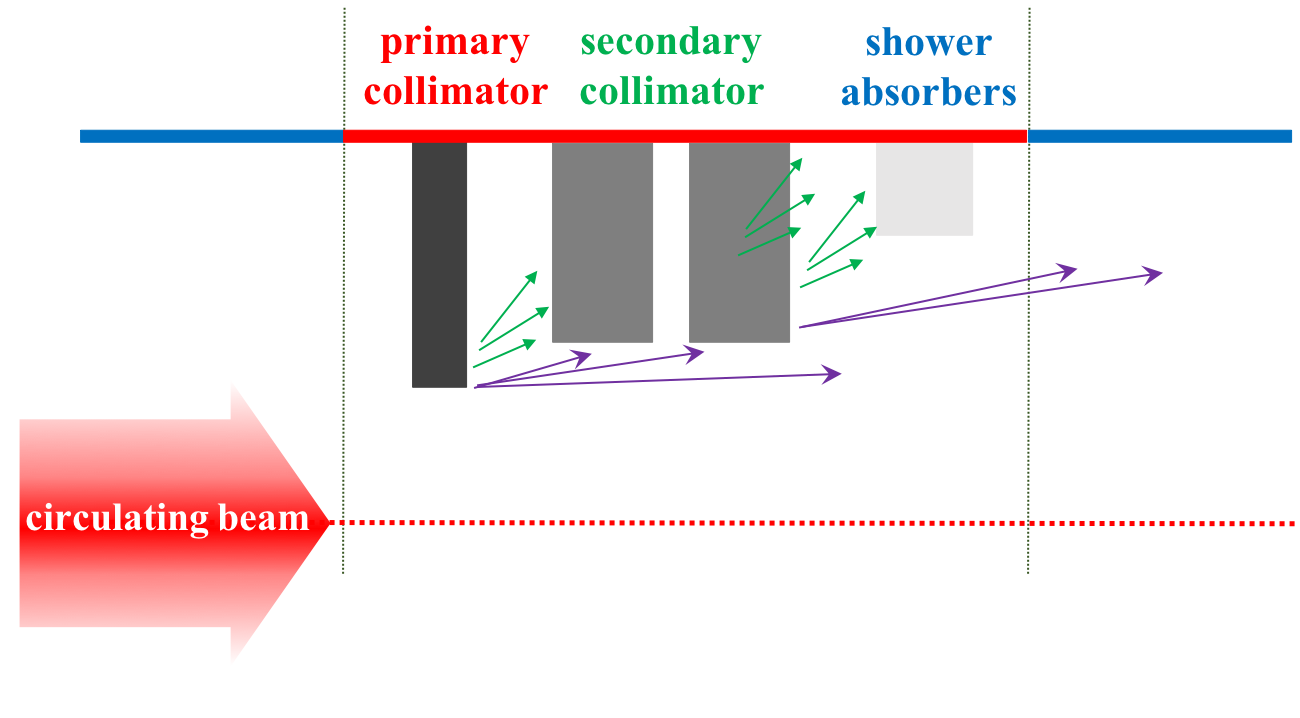
\includegraphics[width=\columnwidth]{passive_halo_control.png}
    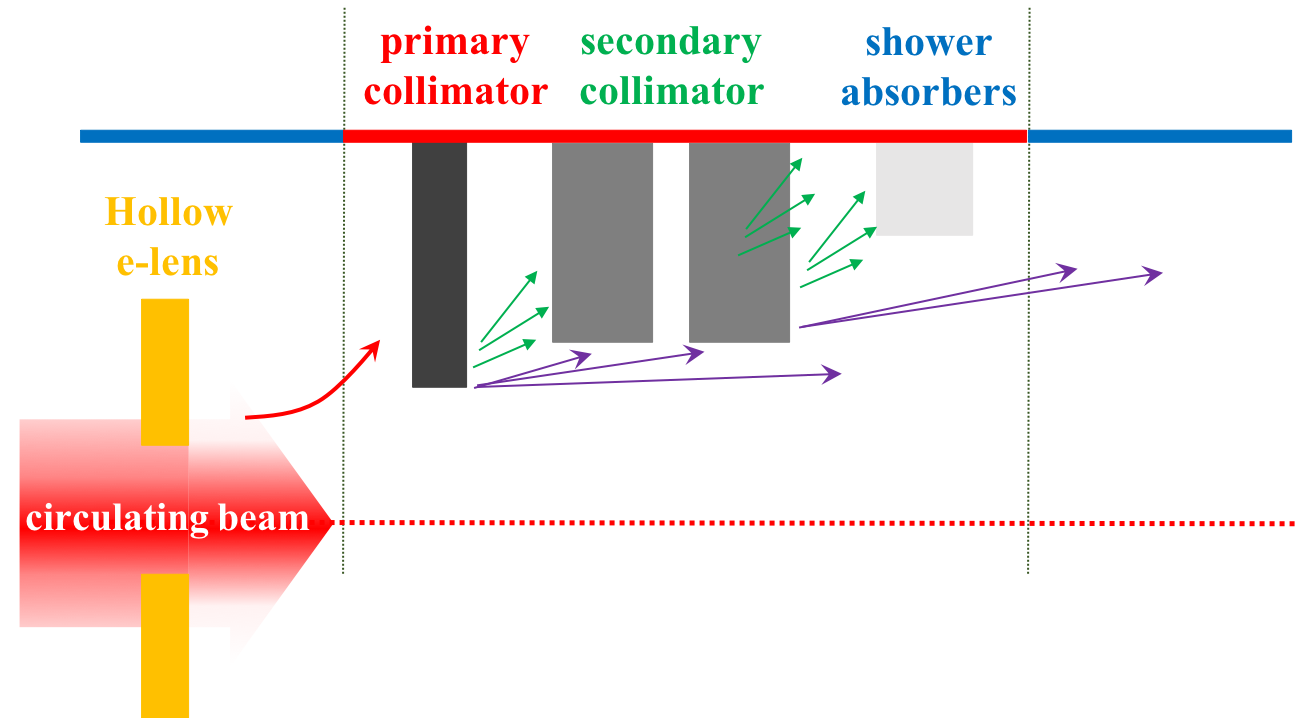
\includegraphics[width=\columnwidth]{active_halo_control.png}
  \end{minipage}
  \hfill
  \begin{minipage}[c]{\columnwidth}
  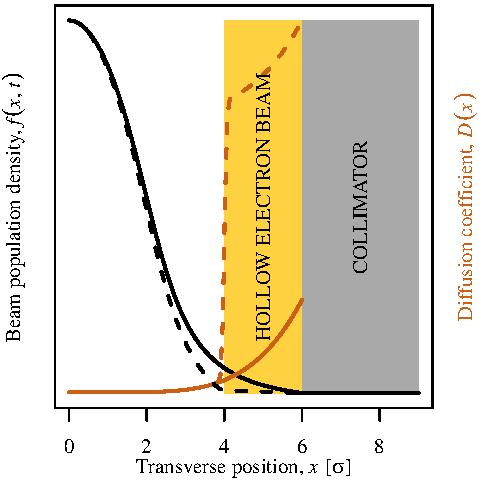
\includegraphics[width=\columnwidth]{diffusion_illustration}
  \end{minipage}
  \caption{Left: Sketch of passive halo control with a conventional
    collimation system (top) and active halo control with the addition
    of a hollow electron lens (bottom). Right: Illustration of a
    simplified model of active diffusion enhancement in the transverse
    plane. The diffusion coefficient as a function of amplitude
    (orange) is enhanced in a specific amplitude region when the
    hollow beam is turned on (from solid to dashed line). A
    corresponding reduction in beam tail population (black) is created
    (from solid to dashed line).}
  \label{fig:active_halo_control} 
\end{figure*}

Considering past, current and future high energy and intensity
colliders, each new machine has represented a considerable leap in
stored beam energy with rising values for future accelerators and
colliders (see Table~\ref{tab:stored_energy}).

Recent measurements at the LHC furthermore show that the tails of the
transverse beam distribution are overpopulated compared to a Gaussian
distribution resulting in a considerable amount of energy being stored
in the beam tails alone. In case of the LHC explicitly around 5\% of
the beam population is stored in the tails above 3.5~$\sigma$ compared
to 0.22\% in case of a Gaussian distribution leading to 19~MJ of
stored energy in the tails in case of nominal LHC parameters and 34~MJ
in case of HL-LHC~\cite{helreview_valentino}. This leads to the
conclusion that a mechanism is needed to deplete the beam tails in a
controlled manner \cite{helreview}.

The most obvious idea is to decrease the collimator gaps or scrape the
tails with a collimator type device. This approach is however not
feasible as it would generate unacceptably large loss spikes due to
the high intensity halo population in the LHC. Most promising are
methods, which increase the diffusion speed in the region of the halo
particles resulting in a smooth and continuous removal of the high
amplitude tails while leaving the core of the beam unperturbed. The
diffusing halo particles are then intercepted by the collimation
system and removed. This concept is also referred to as active halo
control compared to a passive system, which only intercepts the halo
particles without actively controlling the diffusion speed (see
Fig.~\ref{fig:active_halo_control} for illustration).

In a recent review, the need for such an active halo control system for HL-LHC has been assessed with the conclusion that it would considerably increase the margin and reduce the risk for machine protection compared to the current LHC collimation system being a passive halo control system ~\cite{helreview}. In view of the need of active halo control for HL-LHC and for future high power accelerators like HE-LHC and FCC-hh~\cite{helhcparam2011,fcc_coll_ipac2017}, different active halo control methods have been studied in recent years~\cite{helreview_bruce}, of which the hollow electron lens (HEL) is considered the superior device for the HL-LHC~\cite{helreview}. The beneficial effect of a future HEL for HL-LHC in terms of machine protection and beam collimation can not be, however, deployed at the expenses of the beam core as latter would ultimately lead to a degradation of the performance due to increased particle losses and emittance growth. In this paper, we will concentrate on the assessment in simulations and measurements of possible detrimental effets on the beam core. We will summarize possible sources of perturbations of the proton beam core focusing in particular on the case of pulsed operation and the beam experiments at the LHC conducted in this context.

This paper is structured as follows: Section~\ref{sec:hel} gives an introduction to the concept of HELs and summarizes the design parameters of the HL-LHC HELs. Section~\ref{sec:core} is dedicated to describing the sources of a residual field from the HEL in the core region. Section~\ref{sec:exp} then describes in detail the two beam experiments conducted at the LHC studying the effect of pulsed operation on the proton beam core.

\section{Hollow electron lens for HL-LHC\label{sec:hel}}
\subsection{General Overview\label{sec:hel:intro}}
Electron lenses produce DC or pulsed low energy electron beams, where the electron beam is generated in an electron gun, then guided and confined along a straight section by strong solenoids and finally dumped onto a collector. As an example the conceptual design of the HL-LHC HEL is shown in Fig.~\ref{fig:hel_layout}.
\begin{figure}[h]
	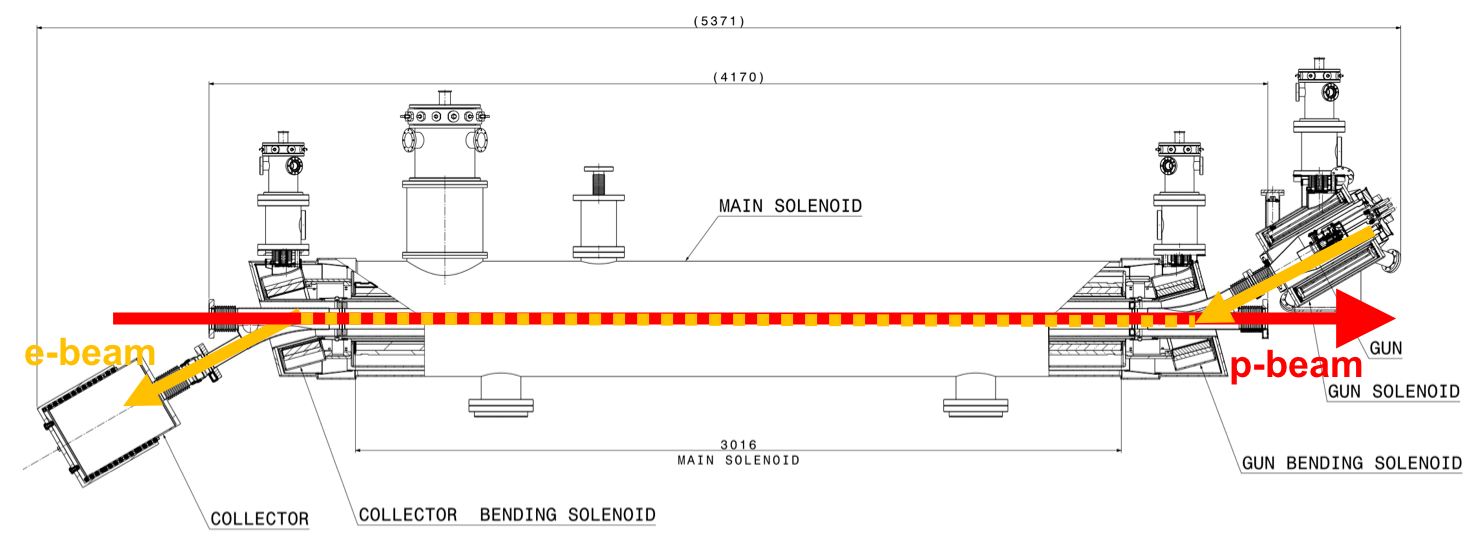
\includegraphics[width=1.0\linewidth]{hel_layout_epbeam}% Here is how to import EPS art
	\caption{\label{fig:hel_layout} Layout of HL-LHC HEL. Courtesy of CERN EN-MME group.}
\end{figure}

\begin{figure}[b]
	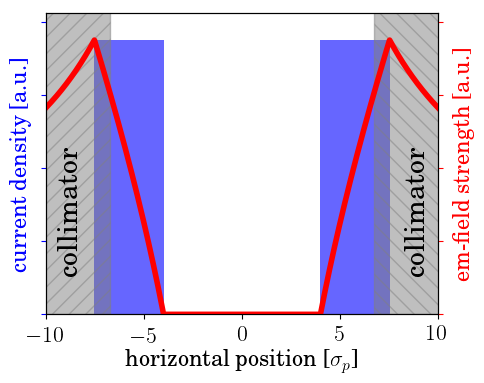
\includegraphics[width=0.8\linewidth]{kick_hel_lhc_no_grid}% Here is how to import EPS art
	\caption{\label{fig:hel_field} Illustration of the hollow electron beam distribution (blue), the kick experienced by the proton beam (red) and the collimators (gray).}
\end{figure}
The circulating beam, in case of the LHC the proton beam, is then affected by the electromagnetic field of the electron beam. For the application of active halo control, the electron beam needs to generate an electromagnetic field at the location of the halo particles while leaving the core unperturbed. This field distribution can be achieved by using a uniform hollow distribution in radius $r=\sqrt{x^2+y^2}$ with inner radius $R_1$ and outer radius $R_2$. In this case, the circulating proton beam experiences a radial kick $\theta(r)$
\begin{equation}\label{eq:field_1}
\theta(r)=\frac{f(r)}{(r/R_2)}\cdot \theta_{\rm max},
\end{equation}
where $f(r)$ is a shape function with
\begin{equation}\label{eq:field_2}
f(r) =
\begin{cases} 0 &,\quad r< R_1,\\
\frac{r^2-R_1^2}{R_2^2-R_1^2} &,\quad R_1 \leq r < R_2,\\
1 &,\quad R_2 \leq r
\end{cases}
\end{equation}
and $\theta_{\rm max}=\theta(R_2)$ is the maximum kick angle given by
\begin{equation}\label{hel_kick_max}
\theta_{\rm max} = \theta(R_2) = \frac{2LI_T(1\pm\beta_e\beta_p)}{4\pi\epsilon_0  \cdot \left(\frac{p_0}{q}\right)_p \cdot \beta_e\beta_p c^2}\cdot\frac{1}{R_2},
\end{equation}
with $L$ the length of the HEL, $I_T$ the total electron beam current, $\beta_{e}$ and $\beta_{p}$ the relativistic $\beta$ of electron and proton beam, $\frac{q}{p_0}=\left(B\rho\right)_p$ the magnetic rigidity for the proton beam reference particle, $c$ the speed of light and $\epsilon_0$ the vacuum permittivity. The distribution together with the resulting kick are illustrated in Fig.~\ref{fig:hel_field}. The $\pm$-sign in Eq.~\ref{hel_kick_max} represents the two cases of the electron beam traveling in the direction of the proton beam ($v_e v_p>0$) leading to ``$-$" or in the opposite direction ($v_e v_p<0$) leading to ``$+$". For hollow electron beam collimation, the beams are chosen to counterrotate. Assuming HL-LHC and HEL design parameters (see Table~\ref{tab:hllhc_param}--\ref{tab:hel_param}) the maximum kick of the HEL is:
\begin{equation}\label{eqn:helkick}
\theta_{\rm max,B1} = 392~\rm{nrad}
\end{equation}
%\begin{eqnarray}
%\theta_{\rm max,B1} = 392~\rm{nrad},\\
%\theta_{\rm max,B2} = 341~\rm{nrad}.
%\end{eqnarray}
for an inner radius of $R_1=4\sigma_p$, outer radius $R_2=7.5\sigma_p$, peak current of $I_e=$\SI{5.0}{A} and Beam~1 of the LHC. Similar values are obtained for Beam~2.
\begin{table}[t]
	\caption{\label{tab:hllhc_param}%
		HL-LHC design parameters at top energy \cite{hlcdr} and parameters relevant in connection with the HEL. Optics parameters at HEL are based on a position of the HEL of $-40$~m for Beam~1 (B1) and $+40$~m for Beam~2 (B2) from IP4 using HL-LHC optics V1.3 with $\beta^{*}=0.15$~m \cite{hlv13}.
	}
	\begin{ruledtabular}
		\begin{tabular}{lccc}
			Beam parameters & Value(B1) & Value(B2) & Unit\\
			\colrule
			Beam energy  $E_{p}$  &  \multicolumn{2}{c}{7} & TeV\\
			Number of bunches $n_b$ & \multicolumn{2}{c}{2748} & - \\
			Number of particles per bunch $N_b$ & \multicolumn{2}{c}{$2.2\times 10^{11}$} & -\\
			Normalized emittance $\epsilon_{N,x/y}$ & \multicolumn{2}{c}{2.5} & $\mu$m\\
			Bunch spacing & \multicolumn{2}{c}{25} & ns\\
			\colrule
			\multicolumn{4}{l}{Optics paramters at HEL (Beam~1) \footnote{As the Twiss parameters at IP4 do not change during the entire squeeze, and IP4 and the HEL are only separated by a drift space, the Twiss parameters stay constant also at the HEL during the entire squeeze.}} \\
			\colrule
			$\beta_{x}$ at HEL  & 197.5 & 280.6 & m\\
			$\beta_{y}$ at HEL & 211.9 & 262.6 m\\
			Dispersion $D_{x}$ at HEL & 0.0& 0.0 & m\\
			Dispersion $D_{y}$ at HEL & 0.0& 0.0 & m\\
			Proton beam size $\sigma_{p,x}$ at HEL & 0.26 & 0.31& mm \\			
			Proton beam size $\sigma_{p,y}$ at HEL & 0.27 & 0.30 &mm \\
			\multicolumn{4}{l}{scraping position}\\ \hspace{1cm}$\sigma_{p}=\max(\sigma_{p,x},\sigma_{p,y})$ & 0.27& 0.31 & mm\\
		\end{tabular}
	\end{ruledtabular}
\end{table}
\begin{table}[t]
	\caption{\label{tab:hel_param}%
		HL-LHC hollow electron lens parameters as in~\cite{hel_cdr}.
	}
	\begin{ruledtabular}
		\begin{tabular}{lcc}
			Geometry & Value& Unit\\
			\colrule
			Length $L$    &  3 & m\\
			% 3-8 sigmap with 3.5 um -> 3.55-9.47 for 2.5 um emittance
			Desired range of scraping positions & 3.5-9.5 &$\sigma_p$\\
			\colrule
			Magnetic fields & & \\
			\colrule
			Gun solenoid, $B_g$ & 0.2-0.4 & T\\
			Main solenoid, $B_m$ & 2-6 & T\\
			Collector solenoid, $B_c$ & 0.2-0.4 & T\\
			Compression factor ($k=\sqrt{B_m/B_g}$) & 2.2-5.5 & -\\
			\colrule
			Electron gun & & \\
			\colrule
			Peak yield $I_e$ at 10~keV & 5.0 & A\\
			Gun perveance $P$ & 5 & $\mu$perv\\
			Inner/outer cathode radius, $R_1/R_2$ & 6.75/12.7 & mm\\
			\colrule
			High voltage modulator & & \\
			\colrule
			Cathode-anode voltage & 10.0 & kV\\
			Rise time (10\%-90\%) & 200 & ns \\
			Repetition rate & 35 & kHz
		\end{tabular}
	\end{ruledtabular}
\end{table}

\subsection{Operation modes and effects on the beam core\label{sec:hel:core}}
For the HEL two modes of operation are currently under consideration, the DC mode as standard operation mode and the pulsed mode. The main benefit of pulsed HEL operation is the increase in halo removal rates which might become essential as in ideal operation conditions featuring low non-linearities, in particular low chromaticity and octupole current, the DC mode is not effective~\cite{hel_halo_hllhc_fitterer,hl_halo_ipac2017}. 
For this purpose, two different pulsing patterns are thus considered for the HL-LHC:
\begin{itemize}
	\item \textbf{random excitation:} The electron gun voltage is modulated between:
	\begin{eqnarray}
	U_{\mathrm{e-gun}}&=&a\cdot U_{\mathrm{max}}\\
	& &+(1-a)\cdot \mathrm{ran}(0,1)\cdot U_{\mathrm{max}}
	\end{eqnarray}
	with $U_{\mathrm{max}}$ the maximum voltage in DC operation, $a$ the modulation strength with $a\in[0,1]$, and $\mathrm{ran}(0,1)$ a uniformly distributed random number between~[0,1].
	\item \textbf{resonant excitation:} The HEL is switched on only every $k^{\mathrm{th}}$ turn. The excitation can then be represented by:
	\begin{eqnarray}\label{intro:eqn:1}
	f(t)&=&\sum_{n=-\infty}^{+\infty}\delta(t-n\cdot(kT)),
	\end{eqnarray}
	where $n$ is the turn number and $T$ the revolution time, and its Fourier series by:
	\begin{eqnarray}\label{intro:eqn:2}
	f(t)=\Sh_{kT}(t)
	&=&\frac{1}{kT}\sum_{n=-\infty}^{+\infty}e^{2\pi i f_nt} \\
	& & \quad \text{with} \ f_n=\frac{n}{k}f_{\rm rev},
	\end{eqnarray}
	where $\Sh_{kT}$ is the Dirac comb. As can be seen from the Fourier series, $k^{\mathrm{th}}$~turn pulsing in general drives $k^{\mathrm{th}}$ order resonances \cite{md_sim_hel_res_ex_fitterer}. Historically, the $k^{\mathrm{th}}$~turn pulsing was used in regular operation in the Tevatron for abort cleaning \cite{hel_tevatron_abortgap_zhang}.
\end{itemize}

As depicted in Fig.~\ref{fig:hel_field} and in evidence from Eqs.~\ref{eq:field_1}--\ref{eq:field_2}, the field at the beam core vanishes in case of an ideal HEL. Effects on the beam core thus only arise from imperfections, where possible sources are the bends of the HEL (see Section~\ref{core:sec:1}), as here the electron beam crosses directly the proton beam, and distortions in the electron beam profile (see Section~\ref{core:sec:2}). Both sources result in non-linear kicks~\cite{hel_bends_stancari,hel_model_polynomial_morozov}. In DC operation, these non-linear kicks stay in the shadow of the non-linearities otherwise present in the machine if the electron beam is kept at a decent quality. Tolerances on imperfections are therefore not particularly stringent and of no concern. The picture changes significantly in case of pulsed operation, in which case the electron gun voltage is modulated using a white or colored noise spectrum. If the electromagnetic field of the HEL does not vanish at the proton beam core, noise is transferred not only to the halo particles, as intended, but also to the beam core. Tolerances on the residual field in this case rapidly become much more stringent than in the case of DC operation. Studies of the effect of the HEL on the beam core therefore focus on this mode of operation which will also be the main subject of this paper.


%In comparison, the random excitation mode is the most effective and operationally easiest pulsing mode, but also the most stringent in terms of tolerances on the residual field at the proton beam center as it induces white noise exciting all beam frequencies. As the resonant excitation acts on specific resonances, the pulsing pattern has to be chosen according to the machine and beam parameters. On the one hand, this makes the operation more difficult as one has to find the most efficient $k^{\mathrm{th}}$~turn pulsing for each operation mode, on the other hand, it also relaxes the tolerances on the residual field at the beam core as, depending on the machine and beam configuration, it might be possible to find a resonant excitation pattern, which mainly affects the halo and not the beam core.

\section{Sources of residual field in the proton beam core region and first order estimates\label{sec:core}}
With the current HEL layout as shown in Fig.~\ref{fig:hel_layout}, parasitic kicks on the proton beam core can arise in the central region due to profile imperfections in the electron beam and at the entrance and exit of the HEL, where electron and proton beam overlap. Currently, no HEL is installed in the LHC, and the kick on the proton beam core must therefore be emulated with the help of other devices already installed in the LHC. For this purpose the kick is approximated to first order by a dipole kick. During the experiments presented in this paper, the dipole kick with the corresponding excitation pattern could then be applied with the LHC transverse damper as will be described in detail in Section~\ref{sec:adt}. As will be shown in Sec.~\ref{core:sec:1} and \ref{core:sec:2}, the expected kick to first order from the HEL bends is estimated to be~(Eq.~\ref{eqn:kick_bends}):
\begin{equation}
	\Delta x'_{\rm{bends}},\Delta y'_{\rm{bends}}\approx \SI{0.5}{nrad},
\end{equation}
and for the central region due to profile imperfections~(Eq.~\ref{eqn:kick_central}):
\begin{equation}
	\Delta x'_{\rm{central \ region}}, \Delta y'_{\rm{central \ region}} \approx \SI{20}{nrad} % this should be rounded to the same number of digits as the 0.5nrad
\end{equation}
where the current HEL design parameters are used (see Table~\ref{tab:hllhc_param}--\ref{tab:hel_param}). The contribution from the central region is clearly dominating.

\subsection{Uncompensated kicks from HEL bends}
\label{core:sec:1}
As reference for the estimate of the dipole component originating from the HEL bends, the symplectic map derived in \cite{hel_bends_stancari} is used. In this case the HEL bends are modeled as a bent cylindrical pipe with a static charge distribution of 1~A and 5~keV electrons deflected in the horizontal plane, where the parameters were her still based on the old gun design for the Tevatron electron lens \textcolor{red}{Giulio, is this correct?}. In case of an U-shaped HEL, the transverse dipole kicks at entrance and exit add up, while for a S-shape the kicks compensate each other. For this reason a S-shape has been chosen for the HL-LHC HEL (see Fig.~\ref{fig:hel_layout}). Assuming and S-shaped HEL, uncompensated kicks therefore only arise from imperfections, which can originate from profile imperfections and current fluctuations. As a first estimate, we assume in this paper 10\% fluctuations between the entrance and exit and, in addition, that the kicks from entrance and exit due to these imperfections add up. Using the electric field calculations in \cite{hel_bends_stancari}, the maximum values for the integrated electric field are then
\begin{equation}
\int_{z_1}^{z_2} E_{x,y} dz= 10 \ \mathrm{kV}.
\end{equation}
%given an \SI{1}{A}, \SI{5}{keV} electron beam.
%For \SI{7}{TeV} protons and neglecting magnetic effects, this yields a kick of:
%\begin{equation}
%\Delta x'=\Delta y'= \SI{1.4}{nrad},
%\end{equation}
%Scaling to the HEL design parameters of a \SI{5}{A} and \SI{10}{keV} electron beam (Table~\ref{tab:hel_param}), one obtains:
%\begin{equation}
%\int_{z_1}^{z_2} E_{x} dz= 36 \ \mathrm{kV} \Rightarrow \Delta x'= \q{5.1}{nrad}
%\end{equation}
Neglecting magnetic effects and scaling to HL-LHC and HEL design parameters (Tables~\ref{tab:hllhc_param}--\ref{tab:hel_param}) yields a kick of \cite{md_sim_hel_res_ex_fitterer}:
\begin{equation}
\int_{z_1}^{z_2} E_{y} dz= 36 \ \mathrm{kV} \Rightarrow \Delta y'= \q{5.1}{nrad}
\end{equation}
Assuming now 10\% fluctuation between entrance and exit kick, the expected kick from the HEL bends is
\begin{equation}\label{eqn:kick_bends}
\Delta x', \Delta y'\approx \q{0.5}{nrad}.
\end{equation}

%\begin{table*}
%	\caption{\label{tab:md_param}%
%		Beam parameters and machine configuration as used in the two resonant excitation experiments in 2016 and 2017 \cite{resexmd2016,resexmd2017}. The plane of the excitation is abbreviated with H for horizontal, V for vertical and H+V horizontal and vertical at the same time.
%	}
%	\begin{ruledtabular}
%		\begin{tabular}{lcc}
%			Parameter & Experiment 2017 & Experiment 2016  \\
%			\colrule
%			beam &\multicolumn{2}{c}{Beam~1} \\
%			beam energy &\multicolumn{2}{c}{injection energy, 450 GeV} \\\hline
%			single bunch intensity &\multicolumn{2}{c}{$0.7\times10^{11}$} \\
%			normalized emittance &\multicolumn{2}{c}{$2.5-3.5~\mathrm{\mu m}$} \\
%			$4\sigma$ bunch length & \multicolumn{2}{c}{1.3~ns}\\
%			$1\sigma$ bunch length & \multicolumn{2}{c}{9.7~cm}\\
%			number of bunches & $3\times72=216$ bunches & $12\times4=48$ single bunches\\
%			& (+ 1 pilot + 12 nominal) & \\\hline
%			injection optics, $\beta^*=11$~m & standard optics 2017 & standard optics 2016\\
%			Landau damping octupoles  & \multicolumn{2}{c}{$I_{\mathrm{MO}}=\pm19.6~\mathrm{A}$, explicitly +19.6 A for MOF circuit and}\\
%			& \multicolumn{2}{c}{-19.6~A for MOD circuit (standard 2016 settings)}\\\hline
%			working point $(Q_x,Q_y)$ & (62.27,60.295) & (64.28,59.31)\\
%			chromaticity $(Q'_x,Q'_y)$ & \multicolumn{2}{c}{(+15,+15)}\\\hline
%			pulsing patterns  & $7^{\mathrm{th}}$~turn H,V,H+V;& $7^{\mathrm{th}}$~turn H;\\
%			& $8^{\mathrm{th}}$~turn H,V,H+V;& $10^{\mathrm{th}}$~turn V;\\
%			& random  H,V,H+V;& \\
%		\end{tabular}
%	\end{ruledtabular}
%\end{table*}

\begin{table*}
	\caption{\label{tab:md_param}%
		Beam parameters and machine configuration as used in the two resonant excitation experiments in 2016 and~2017~\cite{resexmd2016,resexmd2017}. The plane of the excitation is abbreviated with H for horizontal, V for vertical and H+V horizontal and vertical at the same time.
	}
	\begin{ruledtabular}
		\begin{tabular}{lcc}
			Parameter & Experiment 2016 & Experiment 2017  \\
			\colrule
			beam &\multicolumn{2}{c}{Beam~1} \\
			beam energy &\multicolumn{2}{c}{injection energy, 450 GeV} \\\hline
			single bunch intensity &\multicolumn{2}{c}{$0.7\times10^{11}$} \\
			normalized emittance &\multicolumn{2}{c}{$2.5-3.5~\mathrm{\mu m}$} \\
			$4\sigma$ bunch length & \multicolumn{2}{c}{1.3~ns}\\
			$1\sigma$ bunch length & \multicolumn{2}{c}{9.7~cm}\\
			number of bunches & $12\times4=48$ single bunches & $3\times72=216$ bunches\\
			&  & (+ 1 pilot + 12 nominal) \\\hline
			injection optics, $\beta^*=11$~m & standard optics 2016 & standard optics 2017\\
			Landau damping octupoles  & \multicolumn{2}{c}{$I_{\mathrm{MO}}=+19.6~\mathrm{A}$ for MOF circuit and}\\
			& \multicolumn{2}{c}{$I_{\mathrm{MO}}=-19.6~\mathrm{A}$ for MOD circuit (standard 2016 settings)}\\\hline
			working point $(Q_x,Q_y)$ & (64.28,59.31) & (62.27,60.295) \\
			chromaticity $(Q'_x,Q'_y)$ & \multicolumn{2}{c}{(+15,+15)}\\\hline
			pulsing patterns  &$7^{\mathrm{th}}$~turn H; &$7^{\mathrm{th}}$~turn H,V,H+V; \\
			& $10^{\mathrm{th}}$~turn V; & $8^{\mathrm{th}}$~turn H,V,H+V; \\
			& &  random  H,V,H+V;\\
		\end{tabular}
	\end{ruledtabular}
\end{table*}

\subsection{Kicks in the central region (main solenoid)}
\label{core:sec:2}

\begin{figure*}
  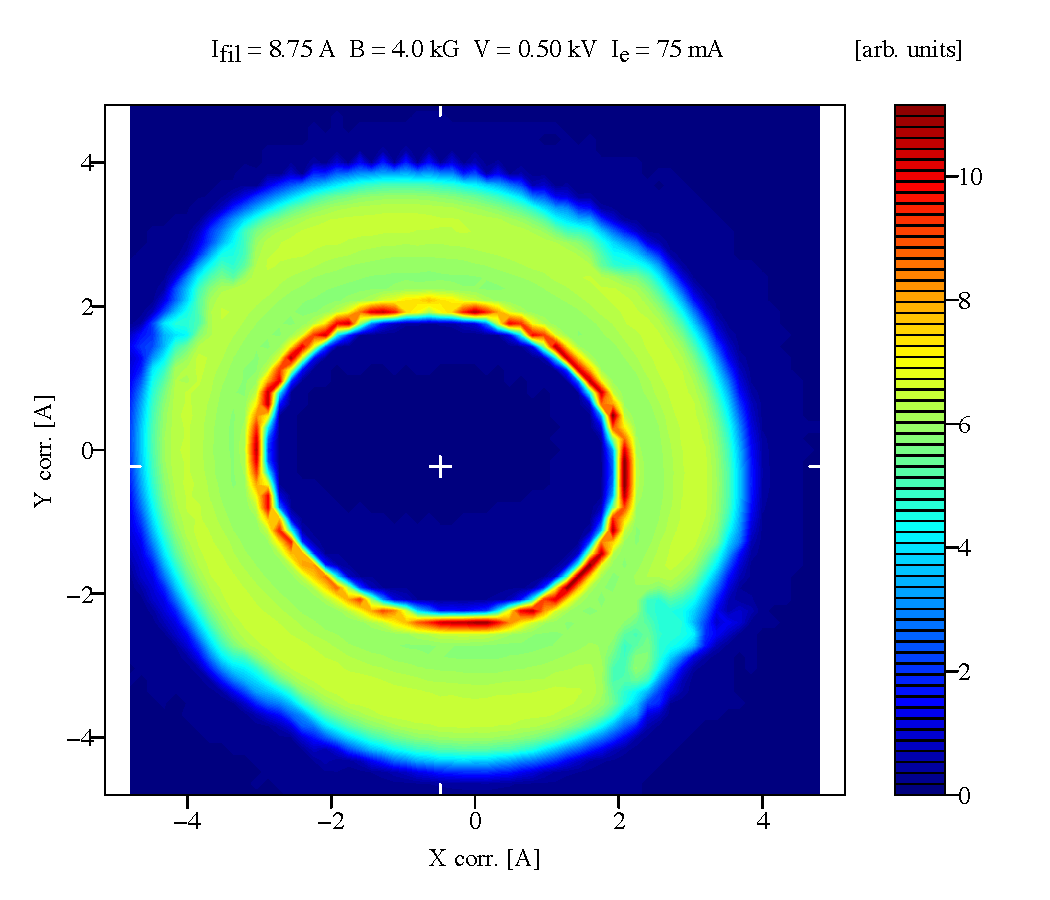
\includegraphics[height=0.9\columnwidth]{CHG1b_170523_8p75A_2-4-2kG_500V_75mA_hires_2D} \hfill
  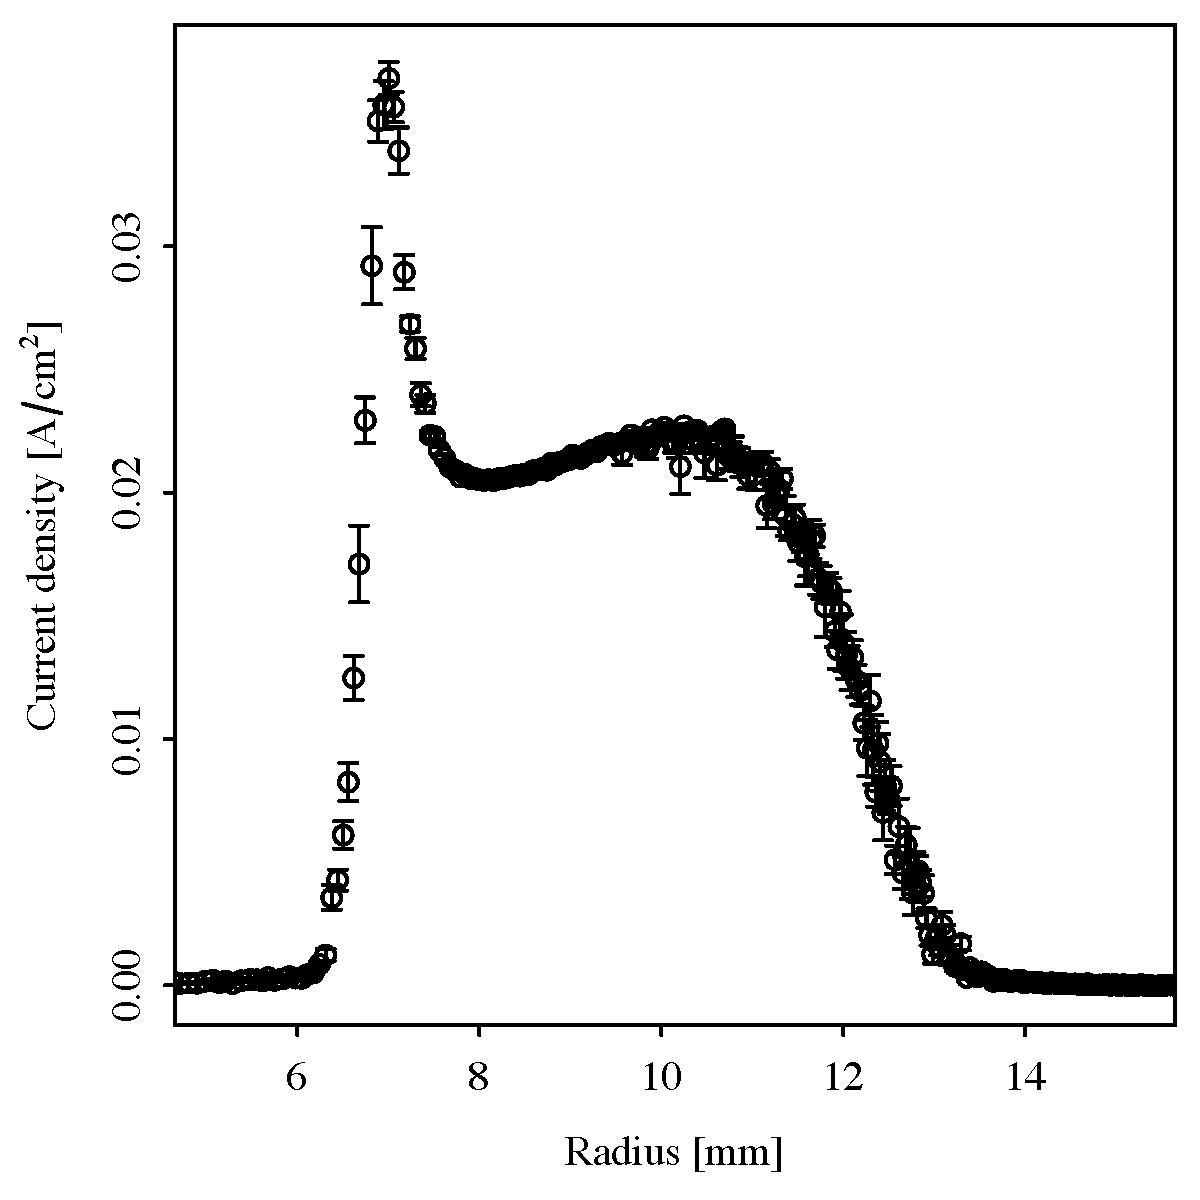
\includegraphics[height=0.9\columnwidth]{CHG1b_170523_8p75A_2-4-2kG_500V_75mA_hires_j-vs-r_binned_nogrid_nolabel}
  \caption{Example of current-density distribution measurements for
    the hollow electron gun prototype CHG1b, taken at the Fermilab
    electron lens test stand in
    2017~\cite{hel_res_field_stancari_2017}: 2-dimensional transverse
    profile measurement (left) and calculated 1-dimensional radial
    projection (right).}
  \label{core:fig:0}
\end{figure*}

\begin{figure*}
  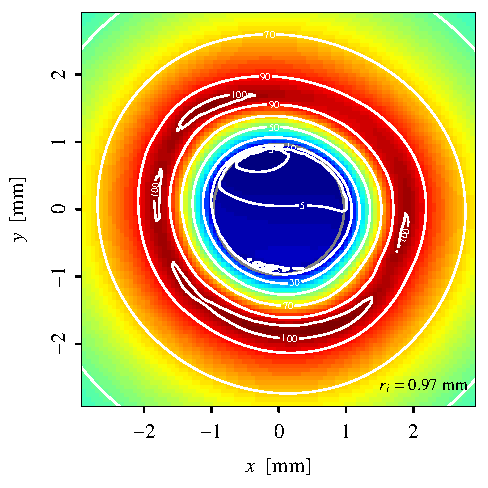
\includegraphics[width=\columnwidth]{CHG1b_170512_8p75A_2-4-2p7kG_500V_76mA_hires_Emap} \hfill
  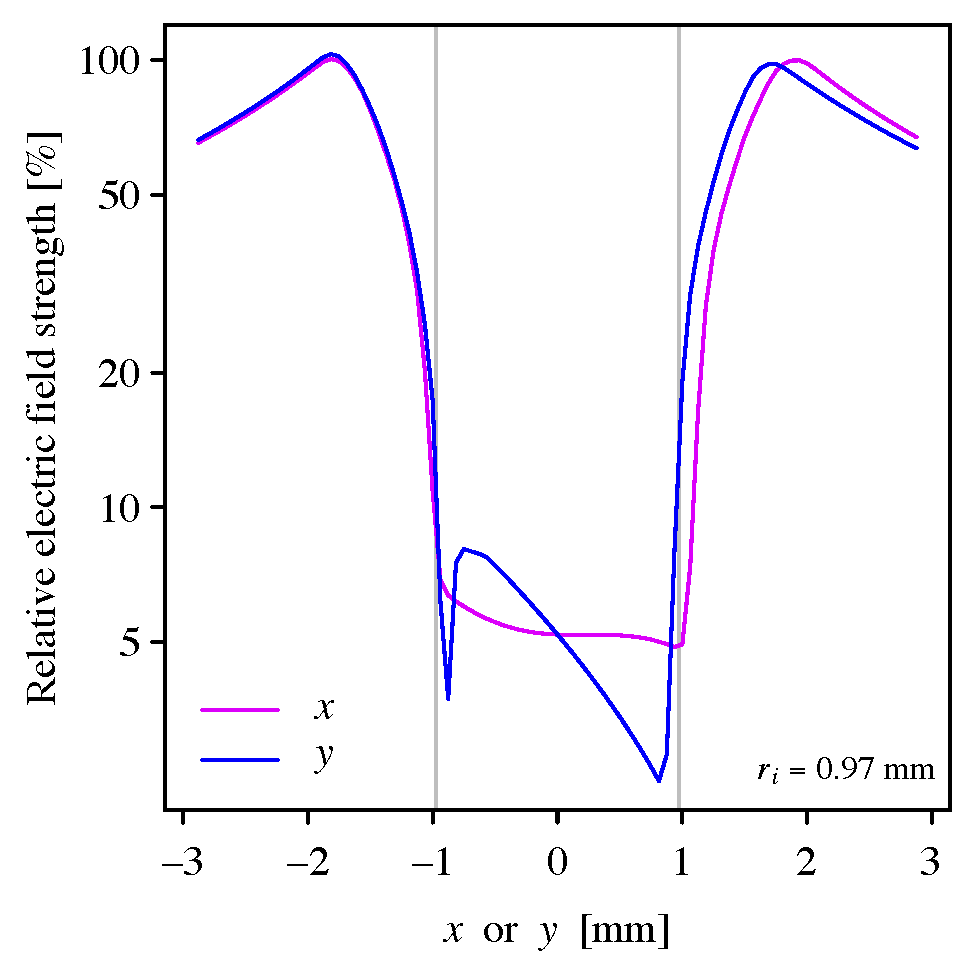
\includegraphics[width=\columnwidth]{CHG1b_170512_8p75A_2-4-2p7kG_500V_76mA_hires_Eslice}
  \caption{Calculated relative electric field for the hollow electron
    gun CHG1b in the transverse $x$-$y$ plane (left) and as
    1-dimensional cuts through the $x$ and $y$ axes (right). The field
    calculations are based on measurements at the Fermilab
    electron-lens test stand combined with Warp calculations of the
    electric potentials and fields in a cylindrical beam pipe.}
\label{core:fig:1}
\end{figure*}

For a perfectly annular and axially symmetric profile, the field in
the region of the proton beam core vanishes. This is expressed by
Eq.~\ref{eq:field_2} and is illustrated in
Fig.~\ref{fig:hel_field}. Fields at the location of the proton beam
core can arise in case of profile imperfections of the electron
beam, in particular if the axial symmetry is broken.

Recently, a hollow electron gun prototype for the LHC (called CHG1b)
was characterized at the Fermilab electron lens test
stand~\cite{hel_test_stand_fnal}. An example of a measurement of the
electron beam current density is shown in Fig.~\ref{core:fig:0}.

In the test stand, only resistive solenoids are available. Through
simulations, one can estimate the fields generated by the compressed
electron beam profile needed for HL-LHC. The measured distribution is
compressed to the inner electron beam radius of 1.24~mm, corresponding
to $4\sigma_p$, as described in Table~\ref{tab:hllhc_param} and
Table~\ref{tab:hel_param}. A distribution with about $65\,000$
particles is generated according to the measured current-density
profile. As boundary condition, the LHC inner beam pipe radius
$b=30$~mm is used. The potential and fields are then calculated with
the particle-in-cell code Warp~\cite{warp}. The resulting relative
electric field strengths are shown in Fig.~\ref{core:fig:1}. The
electric field is obviously proportional to the charge density of
electrons. Its relative strength is rather insensitive to the hollow
beam radii, as long as these remain small compared to the beam pipe
radius. Further details on the measurements and Warp simulations can
be found in Ref.~\cite{hel_res_field_stancari_2017}.

Using these measurements and calculations of the relative electric
field strengths in the transverse plane (Fig.~\ref{core:fig:1}), we
obtain an average field in the hole of

\begin{equation}
  E_{\mathrm{rel}}= 5\%.
\end{equation}

For a maximum kick of 392~nrad, as derived in Eq.~\ref{eqn:helkick},
the estimated dipole kick amplitude at the proton beam core is then

\begin{equation}
  \label{eqn:kick_central}
  \Delta x'_{\rm{central \ region}}, \Delta y'_{\rm{central \ region}} = \SI{20}{nrad}.
\end{equation}

For the scope of this paper, only the approximate magnitude of the
residual dipole kick is considered. In general, the field map,
including its multipolar components, can be parameterized in a
symplectic form, as described for instance in
Ref.~\cite{hel_bends_stancari}, and used in tracking codes to estimate
the effects on the circulating beam.


\section{Experimental and simulation setup\label{sec:exp}}
%put picture on top
\begin{figure*}
	\begin{minipage}[t]{1.0\linewidth}
		\centering
		2016 experiment\\
		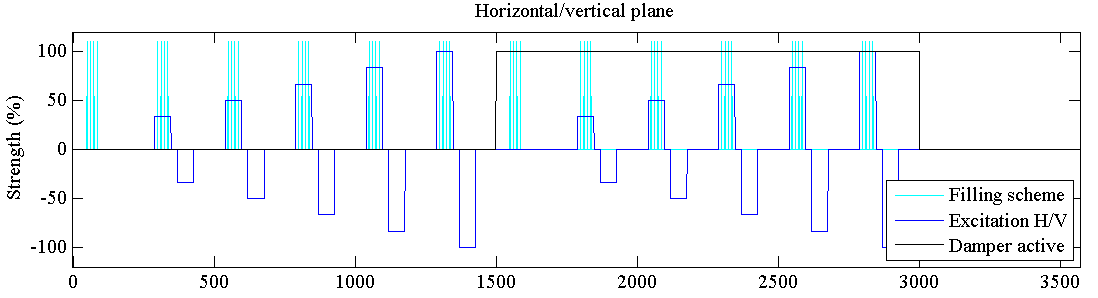
\includegraphics[width=0.9\linewidth]{bunchfilling_2016.png}	
	\end{minipage}
	\begin{minipage}[t]{1.0\linewidth}
		\centering
		$ $\\
		2017 experiment\\
		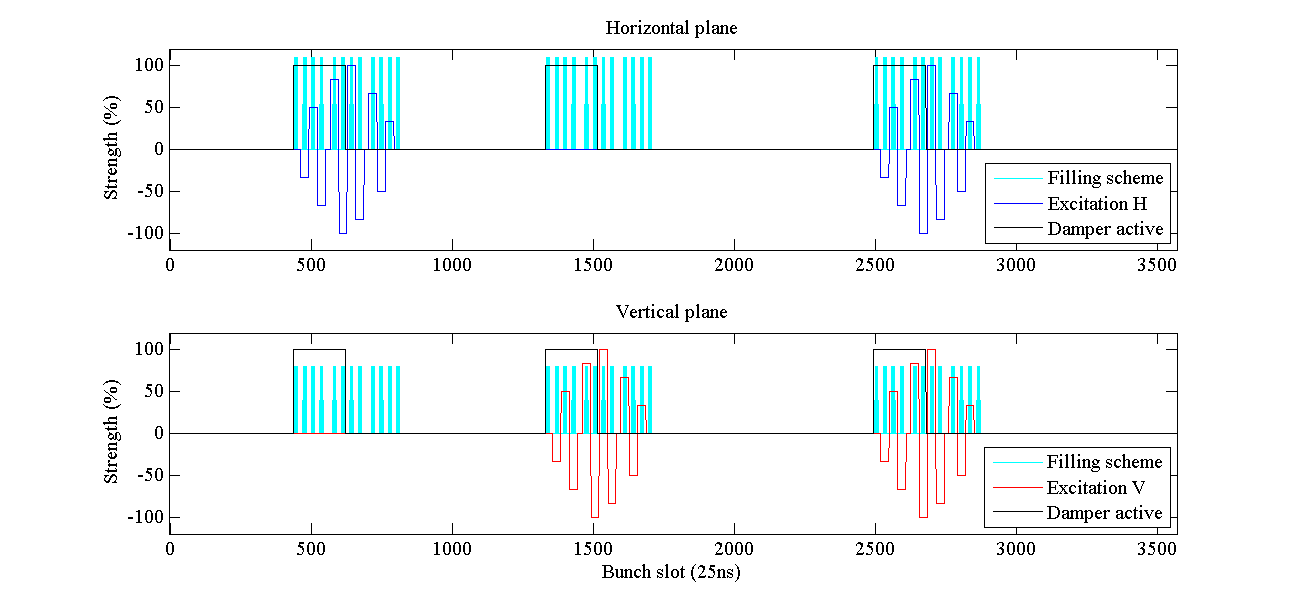
\includegraphics[width=0.9\linewidth]{bunchfilling_2017.png}	
	\end{minipage}
	\caption{\label{fig:fill} Filling and excitation scheme for LHC experiments in 2016 (top) and 2017 (bottom). In 2016 a total of 48~bunches was used and in 2017 a total of 216~bunches. Each bunch is indicated with a cyan vertical bar. The bunches were grouped in sub-groups of 4~for 2016 and 6~for 2017 bunches, where each sub-group experienced the same excitation pattern and amplitude. The excitation amplitude is shown in blue and red. In 2016 the excitation was only applied in one plane. In 2017 more bunches could be injected without compromising machine protection making it possible to test all three planes in one fill.}
\end{figure*}
%put picture on top

\subsection{Overview of LHC experiments\label{sec:exp_sum}}
The experiments at the LHC which are presented in this paper were aiming at deriving tolerances on the residual HEL field at the location of the beam core in case of pulsed operation. In total, two experiments were conducted, the first one in 2016 \cite{resexmd2016} and the second one in 2017 \cite{resexmd2017}. Beam and machine parameters for both experiments are summarized in Table~\ref{tab:md_param}. Preceding the beam experiments, simulations were performed to identify the most effective $k^{\mathrm{th}}$~turn pulsing pattern and yield estimates for losses and emittance growth. The two $k^{\mathrm{th}}$~turn pulsing patterns with the largest effect, one $k^{\mathrm{th}}$~turn pulsing pattern with no effect and the random excitation could then be experimentally tested in the LHC. In order to test the reproducibility of the results at least on the example of one pulsing pattern, the $7^{\mathrm{th}}$~turn pulsing was first tried in 2016 and then repeated in 2017.

During the experiments the losses were measured with the fast beam current transformers (FBCTs) and the emittance and transverse beam profiles with the beam synchrotron radiation telescope (BSRT), where all instruments are capable of delivering bunch-by-bunch data. The analysis of the BSRT profiles is quite involved and we will therefore focus in this paper only on the direct comparison of the profiles. A detailed description of the analysis with more details can be found in \cite{bsrtprofinj} and for the individual experiments in \cite{resexmd2016,resexmd2017}.

\subsection{Excitation with transverse damper and filling scheme\label{sec:adt}}
The primary function of the transverse feedback system in LHC, also referenced to as ADT, is to provide injection oscillation damping and actively damp the coupled bunch instabilities driven by the machine impedance. The main building blocks of the ADT system are stipline pickups at the position Q7 and Q9 at Point~4 of the LHC, connected to the beam position measurement modules at the surface, the digital signal processing modules (mDSPU) and a set of tetrode power amplifiers feeding electrostatic kickers in the RF zone of the LHC~\cite{adt_sum_2008,adt_sum_2011}. Though originally designed to damp the undesired transverse activities only, the damper is being routinely used for sophisticated beam excitations as well thanks to the state of the art digital signal processing hardware. These include among others abort and injection gap cleaning, single bunch excitation for tune and linear coupling measurements and special modes of operation for dedicated experiments at the LHC.

The transverse feedback is in general active during the whole LHC cycle, therefore it is critical that the noise introduced by the system does not contribute to any emittance growth. The typical machine cycle requires a short damping time of ~10-20 turns (high feedback gain) for injection oscillation damping, which is increased during the ramp and collisions to ~50-100 turns (lower feedback gain). It has been demonstrated that noise introduced by the transverse feedback system itself is sufficiently low not to introduce any measurable emittance growth \cite{adt_noise_emit_2017}. All excitation signals referenced to in this paper are digitally synthesized in the damper's digital signal processing units and therefore can be considered as ``noise-free''. This point is important as then the effect on the beam can be attributed entirely to the applied excitation and any effect due to unwanted residual noise can be neglected.

The resonant excitation experiment in 2017 involved simultaneous measurements on three groups of 72 bunches with a dedicated excitation pattern and transverse feedback configuration on each sub-group of 6 bunches. In 2016 a similar configuration was used, but with only 48 bunches in total and sub-groups of 4 bunches. Both schemes are illustrated in Fig.~\ref{fig:fill}. In order to reduce the error of the measurements, the observables are averaged over each sub-group of bunches experiencing the same excitation amplitude, yielding in total 5~different amplitudes $n\Delta A$ with $n=1,\cdots, 5$ plus the references bunch without excitation for each transverse feedback configuration and excitation plane. Furthermore, the experiments were usually split in 3 different parts:
\begin{description}
	\item[Part 1] No excitation is applied in order to allow the distribution to reach an equilibrium state after injection.
	\item[Part 2] The excitation is applied with a first maximum excitation amplitude of $A_{\mathrm{max,1}}=5\Delta A_1$.
	\item[Part 3] The maximum excitation amplitude is further increased to $A_{\mathrm{max,1}} < A_{\mathrm{max,2}}=5\Delta A_2$.
\end{description}
Each part lasted approximately 10-15~minutes, which is considered to be a long enough time window to allow the beam distribution to reach its new equilibrium state. In the plots of the experimental results shown later in the paper, the maximum excitation amplitude is indicated with black horizontal arrows, while the average of each sub-group of bunches with the same excitation amplitude $n\Delta A$ is distinguished with different colors.

The excitation in the horizontal and the vertical plane is generated by a different set of signal processing hardware, however during this experiment the signals were synchronized at a turn level. This means the bunches of the third group (of 72 bunches) experienced the kick in both horizontal and vertical plane during the same turn.

The ADT kicker deflection angle is calculated from the kicker geometry and the excitation voltage on the deflection plates. The excitation voltage used in the experiments is a complicated waveform, generated by a very complex hardware (digital signal processor, chain of transmission lines, low and high power amplifiers). The peak excitation voltage (and subsequently the kick) seen by the beam can be only indirectly measured using the probes on each kicker. The measured values are therefore believed to be known with an error margin of 10-15\% for the experiments in 2017 and 50\% in 2016. The estimate for 2017 is based on only a single measurement and in the future and with more time available the determination of the error would definitely have to be improved. The error in 2016 is estimated from the transverse damper operational parameters. Due to lack of the dedicated machine time no precision calibration was performed. The maximum kick strength reachable with the ADT at injection without risking saturation is 96~nrad. As an example Fig.~\ref{fig:fill_meas} shows the oscillation amplitude of each bunch in both H and V planes captured by the LHC real time transverse activity monitor during the 2017 experiments and an excitation with $8^{\mathrm{th}}$ turn pulsing. The measured activity is well in line with the expected excitation pattern.
\begin{figure*}[h]
	\centering
	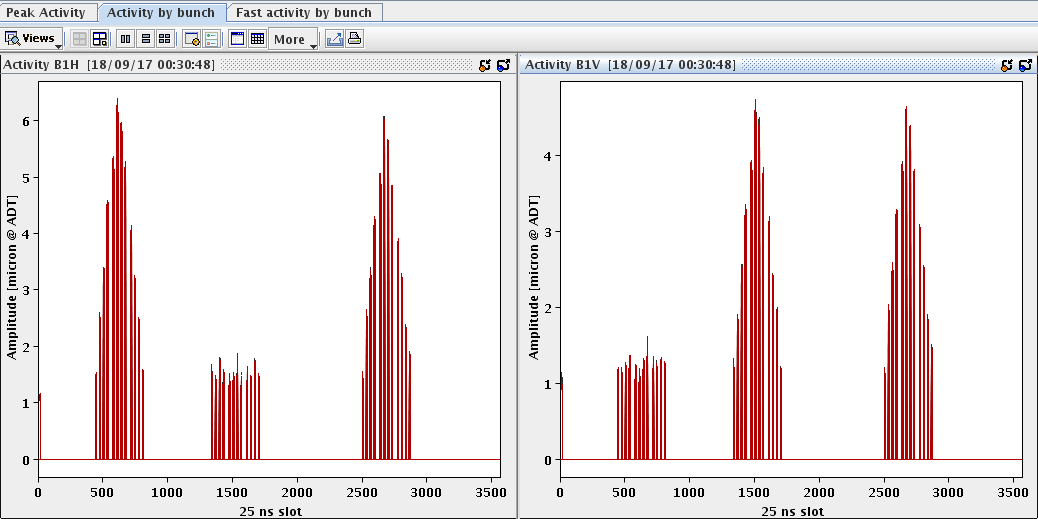
\includegraphics[width=1.0\linewidth]{bunchfilling_measured.png}	
	\caption{\label{fig:fill_meas} Bunch by bunch excitation detected by the real time transverse activity monitor during the 2017 experiment and an excitation with 8th turn pulsing.}
\end{figure*}

\subsection{Overview of simulations\label{sec:sim}}
For the preparation and interpretation of the experiments two different types of simulations were performed:
\begin{enumerate}
	\item tracking of a Gaussian distribution, referred to as ``distribution tracking" in this paper, to obtain loss rates and emittance growth,
	\item Frequency map analysis (FMA) for the visualization of resonances~\cite{fmalaskar}.
\end{enumerate}
For both simulation types, the tracking code Lifetrac \cite{lifetrac} was used. The simulation parameters are summarized in Table~\ref{tab:sim_param}. Further details on the simulations are given in Refs.~\cite{md_sim_hel_res_ex_fitterer,resexmd2017}.
\begin{table}[h]
	\caption{\label{tab:sim_param}%
		Summary of simulation parameters for the distribution tracking and FMA analysis. For details see \cite{md_sim_hel_res_ex_fitterer,resexmd2017}.
	}
	\begin{ruledtabular}
		\begin{tabular}{lcc}
			Parameter & distribution tracking & FMA \\
			\colrule
			beam &\multicolumn{2}{c}{Beam~1} \\
			beam energy &\multicolumn{2}{c}{450 GeV} \\
			emittance & $3.5~\mu$m& $2.5~\mu$m\\
			$4\sigma$ bunch length & \multicolumn{2}{c}{1.3~ns}\\
			$1\sigma$ bunch length & \multicolumn{2}{c}{9.7~cm}\\
			particle & 6D Gaussian & equally spaced grid\\
			distribution &  distribution & in $x,y$ up to $10~\sigma$\\
			&  ($10^4$ particles) & with $\frac{\Delta p}{p_0}=0$\\
			turns tracked & $10^6$ turns & $10^4$ turns \\\hline
			optics & \multicolumn{2}{c}{2016 or 2017 injection optics,}\\
			& \multicolumn{2}{c}{$\beta_{\mathrm{IP1/5}}^*=11$~m}\\
			machine  & standard errors & no errors \\
			imperfections &with $a_1=b_1=0$\footnote{Orbit errors are disabled due to different implementation of the $a_1,b_1$ errors in Lifetrac and MAD-X. $b_2$ errors are adjusted to yield an average (over 60 seeds) peak $\beta$-beat of 15\% as expected from optics measurements in the LHC.} &  \\
			octupoles  & \multicolumn{2}{c}{$I_{\mathrm{MOF}}=+19.6~\mathrm{A}$, $I_{\mathrm{MOD}}=-19.6~\mathrm{A}$}\\
			tune $(Q_x,Q_y)$ & \multicolumn{2}{c}{(64.28,59.31) for 2016,}\\
			& \multicolumn{2}{c}{(62.27,60.295) for 2017}\\
			chromaticity & \multicolumn{2}{c}{(+15,+15)}\\
			$(Q'_x,Q'_y)$ & & \\\hline
			transv. aperture & $5.7~\sigma$ & - \\
			long. aperture & $10~\sigma$ & - \\
		\end{tabular}
	\end{ruledtabular}
\end{table}


\section{Experimental and simulation results\label{sec:simex}}
In the following we will jump forth and back between both experimental and simulation results as the experimental results are best understood on the base of the simulations. In summary, the most efficient pulsing patterns could be successfully predicted in simulations, which we will demonstrate on the example of the 2016 experiments (see Sec.~\ref{sec:pattern}). Afterwards we will present the simulation and experimental results of the tested excitation patterns, explicitly the $10^{\mathrm{th}}$~turn, $7^{\mathrm{th}}$~turn and $8^{\mathrm{th}}$~turn pulsing in Secs.~\ref{sec:simex10}--\ref{sec:simex8} as well as the random excitation in Sec.~\ref{sec:simexran}. As a last chapter, Sec.~\ref{sec:damp}, we will address the influence of the transverse damper in the presence of an external excitation source on emittance, losses and beam distribution.

Quantitative predictions of loss rates and emittance growth proved in general challenging as both observables are influenced in addition by the natural noise present in the LHC, originating for example from vibrations and magnetic field ripple. The observed effect is then the result of the interaction of the external excitation with the natural noise. At injection, this natural noise component is not known and thus presents a very influential but undefined input to the simulations. Beside the natural noise, also collective effects like intra-beam scattering and electron cloud influence the time evolution of emittance and losses. Both are also not taken into account in these simulations, but the effect was minimized during the experiments by choosing an as small as possible bunch intensity of only $0.7\times10^{11}$ protons per bunch.

\subsection{Dependence on the pulsing pattern\label{sec:pattern}}
The effect of each pulsing pattern in comparison to the other patterns can be identified by the means of the loss rate and emittance growth from the distribution tracking. As an example, the simulation results for the 2016 experiment are shown in Fig.~\ref{fig:patternsim} featuring a clear dependence of both parameters on the pattern.
\begin{figure*}[h]
	\begin{minipage}[t]{0.49\linewidth}
		\centering
		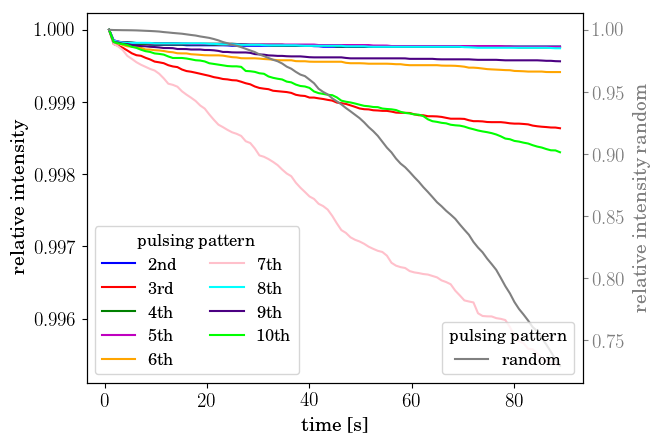
\includegraphics[width=1.0\linewidth]{2016injerra2b2u_pattern_3_5um_intensity.png}
	\end{minipage}
	\begin{minipage}[t]{0.49\linewidth}
		\centering
		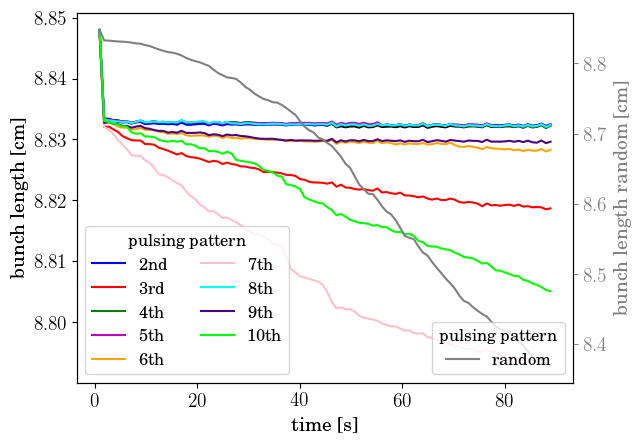
\includegraphics[width=1.0\linewidth]{2016injerra2b2u_pattern_3_5um_sigm.png}
	\end{minipage}	
	\begin{minipage}[t]{0.49\linewidth}
		\centering
		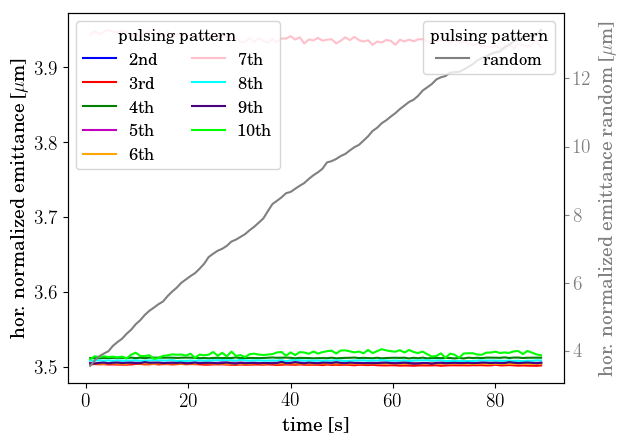
\includegraphics[width=1.0\linewidth]{2016injerra2b2u_pattern_3_5um_emit1.png}
	\end{minipage}
	\begin{minipage}[t]{0.49\linewidth}
		\centering
		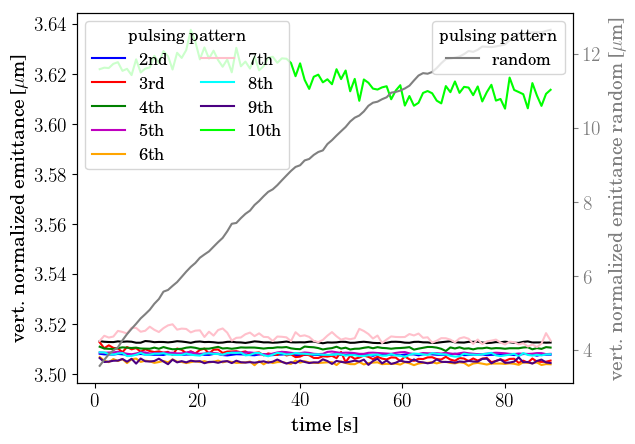
\includegraphics[width=1.0\linewidth]{2016injerra2b2u_pattern_3_5um_emit2.png}
	\end{minipage}	
	\caption{\label{fig:patternsim} Relative intensity (top left), bunch length (top right) and horizontal (bottom left) and vertical (bottom right) emittance for different pulsing patterns obtained from distribution tracking based on the 2016 injection optics with $(Q_x,Q_y)=(64.28,59.31)$ with standard errors. The resonant and random excitation respectively is applied in both planes with an amplitude of 96~nrad. No random noise component is added in addition.}
\end{figure*}

The largest losses are observed for $3^{\mathrm{rd}}$, $7^{\mathrm{th}}$ and $10^{\mathrm{th}}$~turn pulsing and a uniform random excitation. As the bunch length decreases in accordance with the losses, the losses can be mostly associated to off-momentum particles hitting the transverse aperture. Only $7^{\mathrm{th}}$ and $10^{\mathrm{th}}$~turn pulsing as well as random excitation exhibit considerable emittance growth. Compared to any resonant excitation, the random excitation has by far the strongest effect.

The sensitivity to $7^{\mathrm{th}}$ and $10^{\mathrm{th}}$~turn pulsing is also observed in absence of machine errors in which case the only source of non-linearities are sextupoles and octupoles~\cite{md_sim_hel_res_ex_fitterer} suggesting that latter are responsible for the observed sensitivity. The driven resonances are revealed by the FMA analysis shown in Fig.~\ref{fig:patternfma}. The $7Q_x$ resonance is excited in case of the $7^{\mathrm{th}}$~turn pulsing and the $10Q_x$ and $10Q_y$ resonance in case of the $10^{\mathrm{th}}$~turn pulsing. As octupoles can only drive even resonances, the source of the $7Q_x$ resonances are the sextupoles while the octupoles only generate the tune footprint. The other pulsing patterns do not exhibit any increase in losses or emittance growth without magnetic errors and their effect can be thus attributed to the magnetic field errors, implying also the seed chosen for the simulation.
\begin{figure*}[h]
	\begin{minipage}[t]{0.49\linewidth}
		\centering
		no excitation
		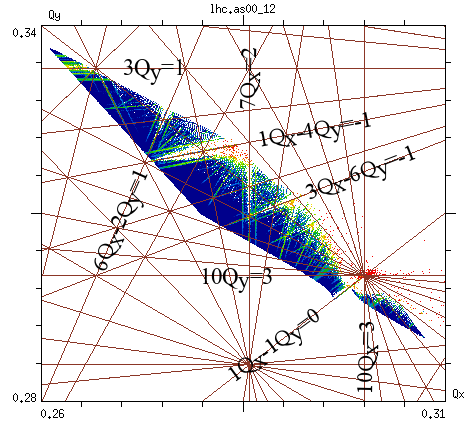
\includegraphics[width=1.0\linewidth]{2016injnocolc15o+19_6noerru_dp0_ord10_annotate.png}
	\end{minipage}
	\begin{minipage}[t]{0.49\linewidth}
		\centering
		$10^{\mathrm{th}}$ H+V
		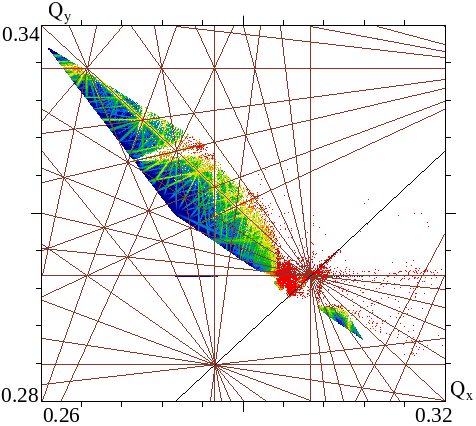
\includegraphics[width=1.0\linewidth]{2016injnocolc15o+19_6noerrut10skhv_dp0_ord10.png}
	\end{minipage}	
	\begin{minipage}[t]{0.49\linewidth}
		\centering
		$7^{\mathrm{th}}$ H
		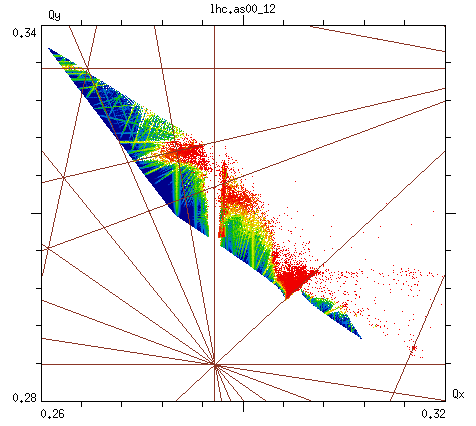
\includegraphics[width=1.0\linewidth]{2016injnocolc15o+19_6noerrut7skh_dp0_ord7.png}
	\end{minipage}	
	\begin{minipage}[t]{0.49\linewidth}
		\centering
		$7^{\mathrm{th}}$ V
		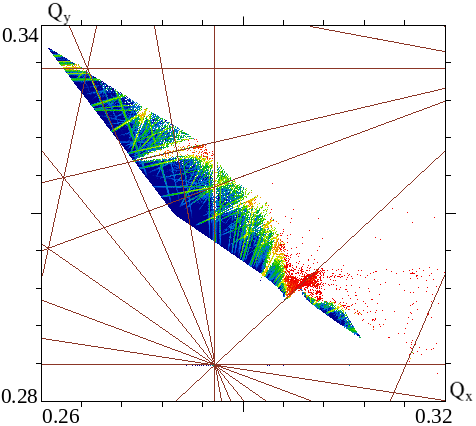
\includegraphics[width=1.0\linewidth]{2016injnocolc15o+19_6noerrut7skv_dp0_ord7.png}
	\end{minipage}
	\caption{\label{fig:patternfma} FMA analysis without excitation (top left) for $10^{\mathrm{th}}$~turn pulsing in H+V (top left) and for $7^{\mathrm{th}}$~pulsing only in H (bottom left) and only in V (bottom right) and  based on the 2016 injection optics with no machine errors and a tune of (64.28,59.31). The excitation is 120~nrad in the corresponding plane. The absence of a strong excitation of any resonance in case of $7^{\mathrm{th}}$~turn pulsing only in V and the strong excitation in case of pulsing only in H confirms the excitation of the $7Q_x$ resonance. For $10^{\mathrm{th}}$~turn pulsing there is in contrast no significant difference between pulsing only in H, only in V or in H+V (see Appendix~\ref{app:sec:10}, Fig.~\ref{app:fig:fma:10}).}
\end{figure*}  

One may have noticed that the emittance in case of the $7^{\mathrm{th}}$ and $10^{\mathrm{th}}$~turn pulsing starts at an increased initial value and then stays almost constant during the entire simulation time, which usually points to an error in the chosen simulation setup. This behavior is however typical for any resonant excitation and can be ascribed to the adjustment of the beam distribution during the first $10^4$ turns to a new equilibrium. As the beam distribution is only dumped every $10^4$ turns, this initial fast adjustment manifests itself in an increased initial emittance value in Fig.~\ref{fig:patternsim}, and also any other simulations over $10^6$ turns presented in this paper. Besides an increased emittance, the new distribution also becomes non-Gaussian. This is illustrated by means of the residual in respect to the Gaussian distribution for $7^{\mathrm{th}}$ and $10^{\mathrm{th}}$~turn pulsing in Fig.~\ref{fig:patternhist}. This initial fast change of the beam distribution is not an artifact of the simulation, but has been, to the knowledge of the authors, also for the first time experimentally observed during the 2016 and 2017 LHC experiments presented in this paper. The timescale of this fast adjustment is in experiments however much slower than predicted in simulations --- on the timescale of minutes compared to seconds. 
\begin{figure*}[t]
	\begin{minipage}[t]{0.49\linewidth}
		\centering
		$7^{\mathrm{th}}$ H+V
		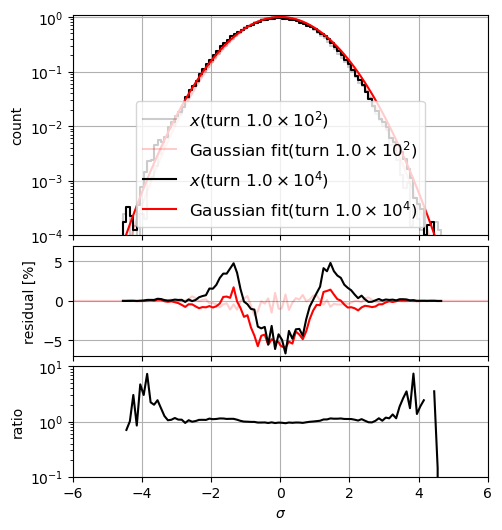
\includegraphics[width=1.0\linewidth]{2016injerra2b2u_t7skhv_3_5um_hist_x.png}
	\end{minipage}
	\begin{minipage}[t]{0.49\linewidth}
		\centering
		$10^{\mathrm{th}}$ H+V
		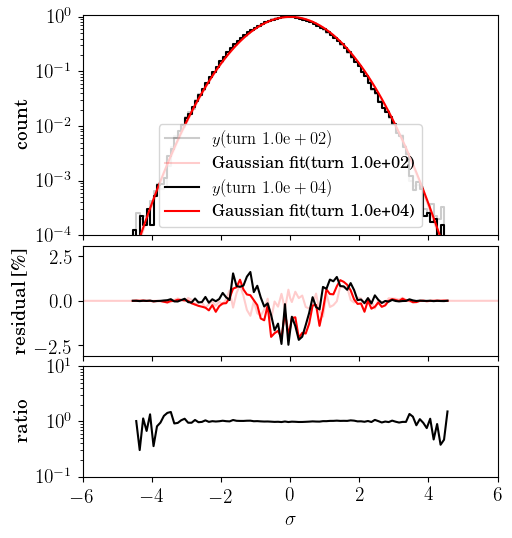
\includegraphics[width=1.0\linewidth]{2016injerra2b2u_t10skhv_3_5um_hist_y.png}
	\end{minipage}	
	\begin{minipage}[t]{0.49\linewidth}
		\centering
		random H+V
		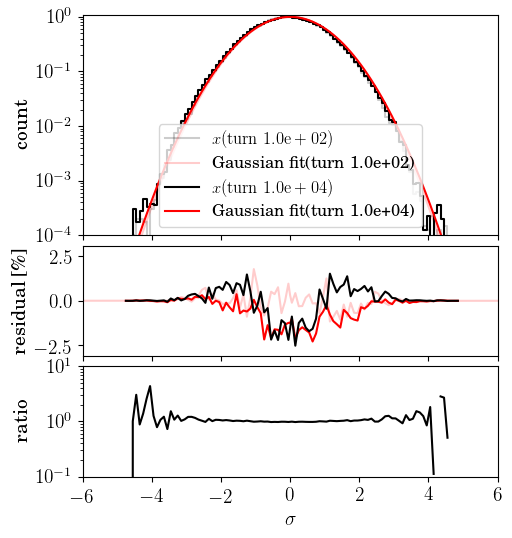
\includegraphics[width=1.0\linewidth]{2016injerra2b2u_ranhv_3_5um_hist_x.png}
	\end{minipage}
	\begin{minipage}[t]{0.49\linewidth}
		\centering
		no excitation
		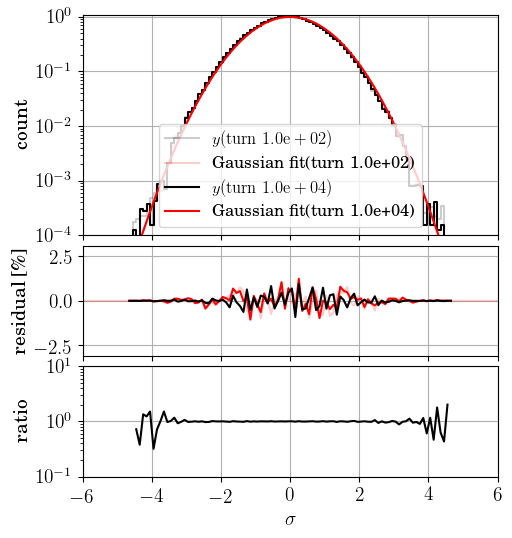
\includegraphics[width=1.0\linewidth]{2016injerra2b2u_3_5um_hist_y.png}
	\end{minipage}	
	\caption{\label{fig:patternhist} Horizontal beam distribution for $7^{\mathrm{th}}$~turn pulsing (top left), vertical beam distribution for $10^{\mathrm{th}}$~turn pulsing (top right) and horizontal (bottom left) and vertical (bottom right) beam distribution for random excitation from distribution tracking simulations based on the 2016 injection optics with $(Q_x,Q_y)=(64.28,59.31)$ and standard errors. The excitation is applied in both planes with an amplitude of 96~nrad. The residual is defined as the final distribution (here after $10^4$~turns) minus the initial distribution (here after $10^2$~turns) as \%, and the ratio as the final distribution divided by the initial distribution. The red line in the plot of the residual is the difference between the Gaussian fit of the distribution and the distribution itself.}
\end{figure*}

In the presence of only a resonant excitation, this modified distribution is stable in simulations with a constant emittance. As we will see later, an increase of the emittance with the applied excitation amplitude is however observed experimentally not matching the prediction by simulations. By adding a random noise component representative for the natural noise present in the LHC, the constant emittance is changed in simulations to an excitation amplitude dependent emittance growth after an initial adjustment phase. In case of random uniform noise, the excitation leads to constant emittance growth without any initial adjustment phase. The interaction with the natural noise source then only results in an underestimation of loss rates and emittance growth as it is basically equivalent to the application of random noise with an increased amplitude. In addition to the experiments presented in this paper, the effect of a random excitation was also studied in a separate experiment at the LHC for the case of colliding beams \cite{md1433_noise_top_energy,md_noise_bbLHC}.

\clearpage

\subsection{$10^{\mathrm{th}}$ turn pulsing\label{sec:simex10}}
The $10^{\mathrm{th}}$~turn pulsing pattern was tested in 2016 with an excitation in the vertical plane only. As this was the first time a resonant excitation was tested in the LHC, only in total 48~bunches could be injected in order to still guarantee the protection of the machine. To test different excitation amplitudes during one fill and have enough statistics, the excitation was therefore only applied in one plane. As described earlier, the experiment started with a period of 12~minutes without excitation in order to let the beam distribution fully adjust to its equilibrium state after injection. Afterwards the excitation was applied with the excitation scheme shown in Fig.~\ref{fig:fill} and a maximum excitation amplitude of $A_{\mathrm{max}}=5\Delta A = 48~$nrad for a total of 11~minutes. The excitation was then further increased to the maximum value reachable without saturation of $A_{\mathrm{max}}=5\Delta A = 96~$nrad and kept for 11~minutes. In both cases, the excitation induced the following changes:
\begin{enumerate}
	\item Increase of the loss rate with the excitation amplitude (Figs.~\ref{fig:10thexp}.
	\item Increase of the emittance growth with the excitation amplitude in the vertical plane but not in the horizontal plane (Fig.~\ref{fig:10thexp}).
	\item Change of the beam distribution for the excited bunches (Fig.~\ref{fig:10thexpprof}).	
\end{enumerate}
As loss rates, emittance growth and beam distribution stayed unchanged for the $4$~reference bunches, the above observations can be also truly associated with the effect of the $10^{\mathrm{th}}$~turn pulsing.
\begin{figure*}[h]
	\begin{minipage}[t]{0.32\linewidth}
		\centering
		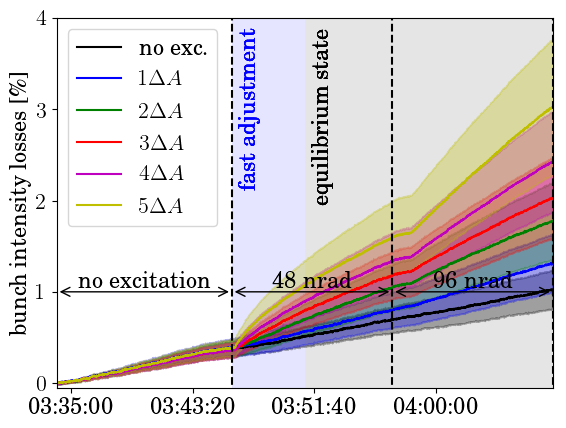
\includegraphics[height=0.75\linewidth]{2016_bunch_intensity_v10th_no_damper_avg.png}
	\end{minipage}
	\begin{minipage}[t]{0.32\linewidth}
		\centering
		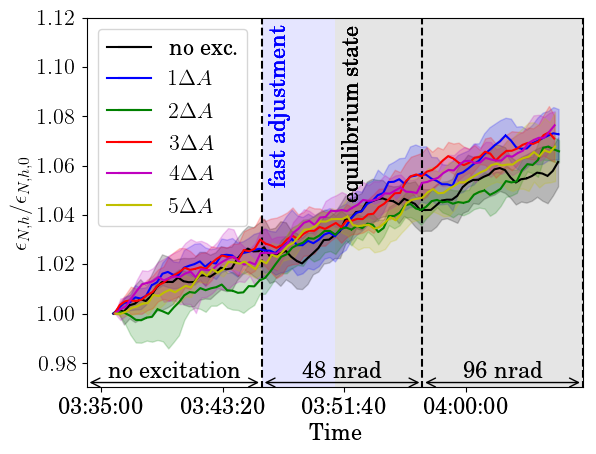
\includegraphics[height=0.75\linewidth]{2016_emith_avg_rel_v10th_no_damper.png}
	\end{minipage}	
	\begin{minipage}[t]{0.32\linewidth}
		\centering
		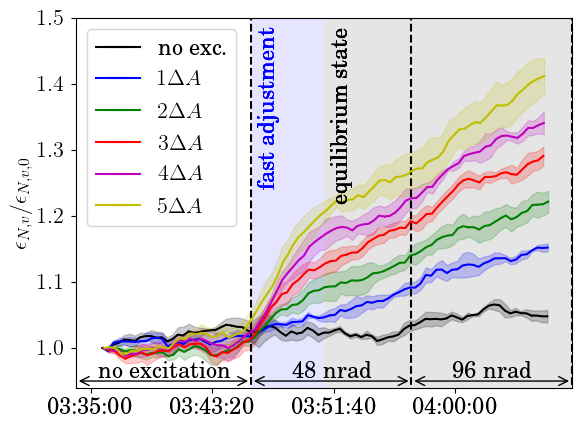
\includegraphics[height=0.75\linewidth]{2016_emitv_avg_rel_v10th_no_damper.png}
	\end{minipage}	
	\caption{\label{fig:10thexp} Relative intensity (top) and relative horizontal (bottom left) and vertical (bottom right) emittance averaged over the bunches experiencing the same excitation amplitude during the 2016 experiments and for $10^{\mathrm{th}}$~turn pulsing in~V. For all bunches the damper was not active. Relative refers here to the normalization to the initial value. For each maximum amplitude $A_{\mathrm{max}}=48$~nrad and 96~nrad indicated with black arrows, the excitation amplitude was linearly increased for each group of 4~bunches (see Fig.~\ref{fig:fill}). The different colored solid lines labeled with $n\Delta A$ are the average over the 4~bunches with the same excitation amplitude together with the $1\sigma$ standard deviation shown as envelope. The area with a blue background indicates the fast adjustment period of the beam distribution transitioning into a new equilibrium state highlighted with a gray background.}
\end{figure*}
These experimentally obtained scalings of the loss rate and emittance growth with the excitation amplitude can be then used for the actual specification of the hollow electron lens.

Besides the numerical determination of tolerances, the vertical emittance actually features indeed the strange and interesting behavior predicted in simulations: a fast adjustment phase of the beam distribution visible as a rapid increase of the emittance followed by the reach of a new equilibrium distribution apparent by a slower continuous emittance growth. These two phases are indicated in Fig.~\ref{fig:10thexp} in blue and black.

\begin{figure*}[h]
	\begin{minipage}[t]{0.49\linewidth}
		\centering
		reference bunch, no excitation
		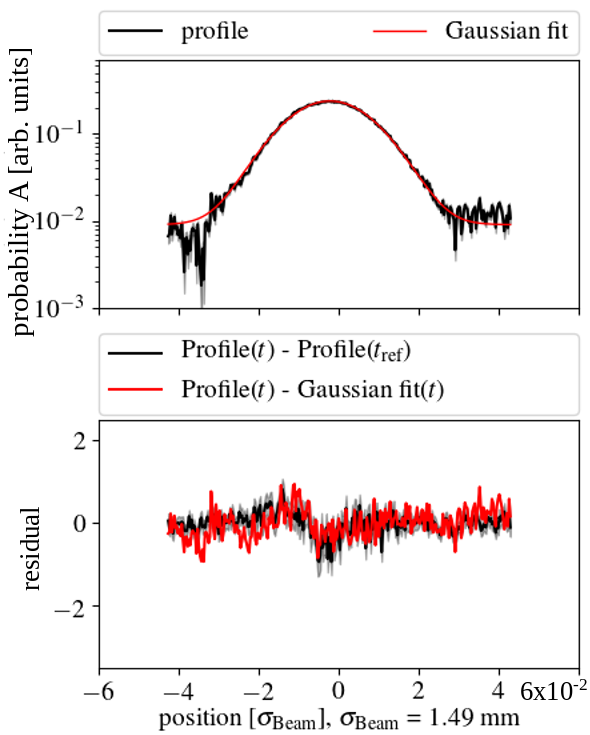
\includegraphics[width=1.0\linewidth]{profile_v_10thv_slot_50.png}
	\end{minipage}
	\begin{minipage}[t]{0.49\linewidth}
		\centering
		excited bunch, $10^{\mathrm{th}}$~turn V		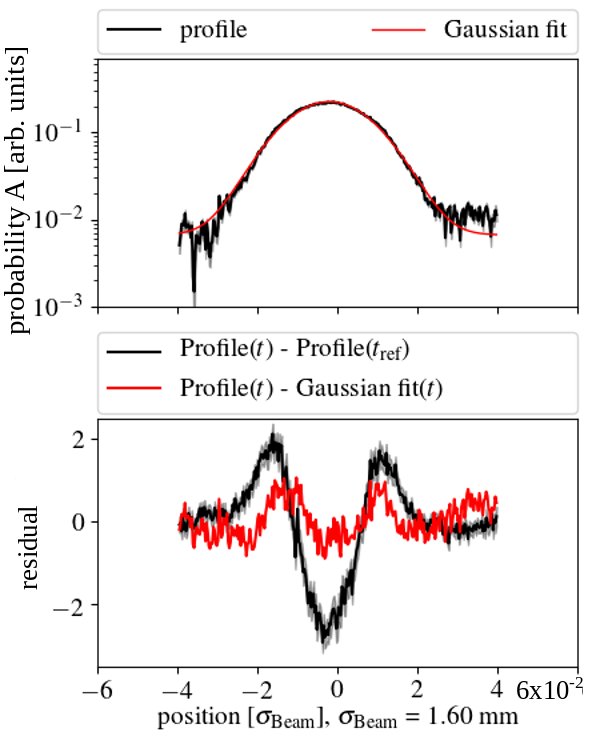
\includegraphics[width=1.0\linewidth]{profile_v_10thv_slot_1300.png}
	\end{minipage}
	\caption{\label{fig:10thexpprof} Vertical beam profiles measured with the Beam Synchrotron Radiation Telescope (BSRT) during the 2016 experiments. The profiles are taken at the end of the $10^{\mathrm{th}}$~turn pulsing in V. For both bunches the transverse damper is not active. The black line in the plot of the residual is the current profile minus the profile before applying the excitation and is a measure for the overall change of the distribution. The red line is the current profile minus its Gaussian fit, which gives and indication for the deviation of the distribution from a Gaussian distribution. For details on the analysis it is referred to \cite{bsrtprofinj}. The distribution of the reference bunch (left), here slot 50, stays unchanged, while the bunch experiencing the maximum excitation (right), here slot 1300, clearly shows a change to a non-Gaussian distribution.}
\end{figure*}
Thanks to the good performance of the Beam Synchrotron Radiation Telescope (BSRT)~\cite{bsrtprofinj}, the distribution changes indirectly observed as changes of the emittance could also be for the first time directly measured. As example Fig.~\ref{fig:10thexpprof} shows the vertical profile of a reference bunch and one bunch experiencing the maximum excitation of $5\cdot\Delta A=A_{\mathrm{max}}=48$~nrad and afterwards 96~nrad. The distribution of the excited bunch not only changes but becomes clearly non-Gaussian, while the reference bunch stays unchanged.
\begin{figure*}[h]
	\begin{minipage}[t]{0.49\linewidth}
		\centering
		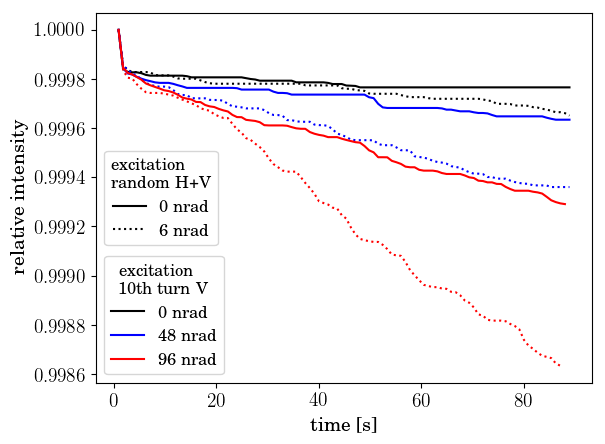
\includegraphics[width=1.0\linewidth]{2016injerra2b2uran1_2e-3_10thV_3_5um_intensity.png}
	\end{minipage}
	\begin{minipage}[t]{0.49\linewidth}
		\centering
		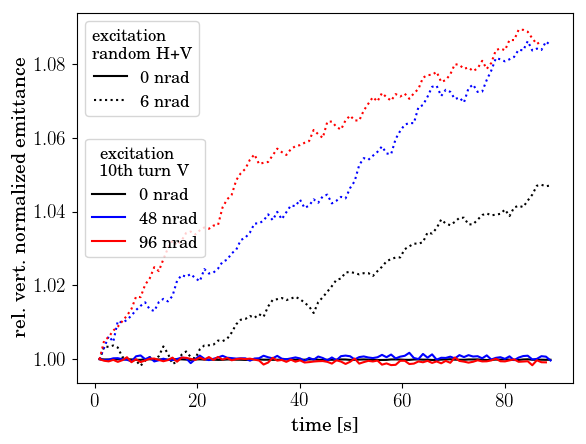
\includegraphics[width=1.0\linewidth]{2016injerra2b2uran1_2e-3_10thV_3_5um_emit2_rel.png}
	\end{minipage}
	\begin{minipage}[t]{0.49\linewidth}
		\centering
		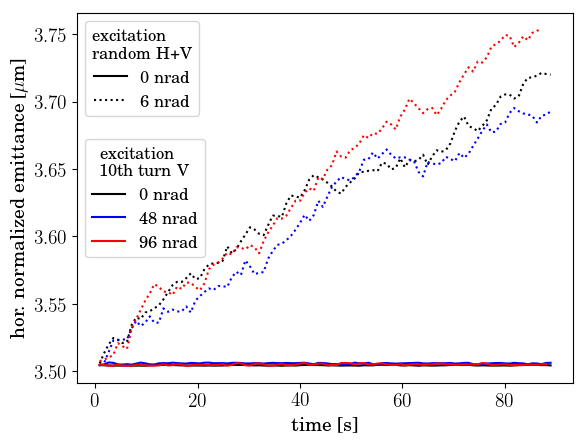
\includegraphics[width=1.0\linewidth]{2016injerra2b2uran1_2e-3_10thV_3_5um_emit1.png}
	\end{minipage}	
	\begin{minipage}[t]{0.49\linewidth}
		\centering
		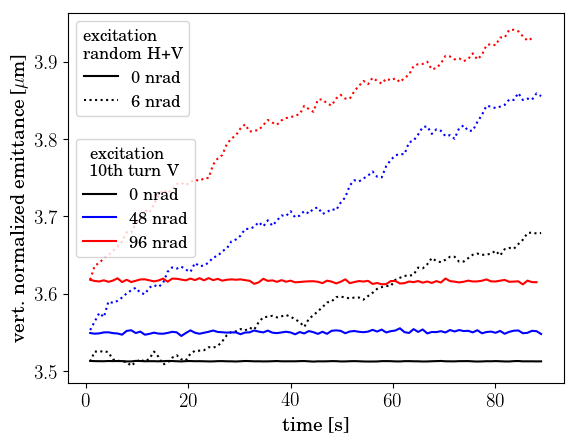
\includegraphics[width=1.0\linewidth]{2016injerra2b2uran1_2e-3_10thV_3_5um_emit2.png}
	\end{minipage}	
	\caption{\label{fig:10thsim} Relative intensity (top left) and relative vert. emittance (top right), and hor. (bottom left) and vert. (bottom right) emittance obtained from simulations (distribution tracking) based on the 2016 injection optics with standard errors and $(Q_x,Q_y)=(64.28,59.31)$. The solid line indicates an excitation with only $10^{\mathrm{th}}$~turn pulsing in V and the dotted line with $10^{\mathrm{th}}$~turn pulsing in V plus a random dipole noise component in H+V of 6~nrad.}
\end{figure*}
The simulation results from the distribution tracking for $10^{\mathrm{th}}$~turn pulsing and without (solid line) and with (dotted line) additional random noise component to emulate the natural noise present in the LHC are shown in Fig.~\ref{fig:10thsim}. As no estimate of the natural noise is available at injection for the LHC, a first estimate is obtained by scaling the estimate for 6.5~TeV \cite{md1433_noise_top_energy,md_noise_bbLHC} by the magnetic rigidity to the injection energy of 450~GeV. This yields a maximum kick amplitude at the transverse damper of approximately
\begin{equation}
\theta_{\mathrm{random,ADT,max}}(\mathrm{450~GeV}) = 6~\mathrm{nrad}.
\end{equation}
As can be seen from simulations, adding a random noise component not only yields the correct qualitative behavior of the emittance but also increases the losses. As the losses are in general underestimated in simulations compared to the experimental results, the discrepancy between simulations and experiment can be thus reduced.  To better compare the experimental results for the two different maximum excitation amplitudes applied for slightly different time intervals and also the simulations conducted for a much shorter interval of only 90~s, we define the relative loss rate $R$:
\begin{equation}\label{eqn:lossrate}
R = \frac{I_{\mathrm{start}}-I_{\mathrm{end}}}{I_{\mathrm{start}}\cdot \Delta t}
\end{equation}
where $I$ is the intensity and $\Delta t$ the time interval during which the excitation with fixed $A_{\mathrm{max}}$ is applied during the experiments or the duration of the simulation respectively. A qualitative comparison of the loss rates obtained in experiments and simulations is shown in Fig.~\ref{fig:10thexploss} featuring a surprisingly good agreement. It should be also kept in mind that the additional random noise component considerably influences the simulation results and as long as it is unknown should be seen more as a fit parameter than a real experimentally confirmed input parameter. The measured loss rates for $A_{\mathrm{max}}=48$~nrad and $A_{\mathrm{max}}=96$~nrad should furthermore follow the same scaling. Instead the loss rates for the same excitation amplitude are smaller for $A_{\mathrm{max}}=96$~nrad compared to $A_{\mathrm{max}}=48$~nrad. That losses and also emittance growth for a fixed excitation amplitude do not exactly agree for both experiments, is a general tendency observed in all experiments. As the second excitation however starts from an already by the previous excitation changed beam distribution, the difference is however not surprising and can be explained by this difference in initial conditions. For checking the reproducibility of the results in a possible future experiment, it would be interesting to see if the same loss rates are measured if for each $A_{\mathrm{max}}$ a new fill is used. 
\begin{figure}[h]
		\centering
%		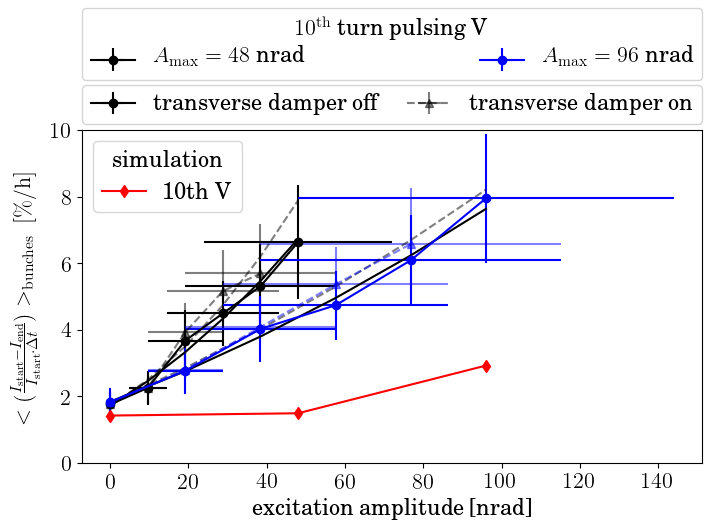
\includegraphics[width=0.8\linewidth]{2016_scale_amp_10v_ran_lbllong_sim.png}
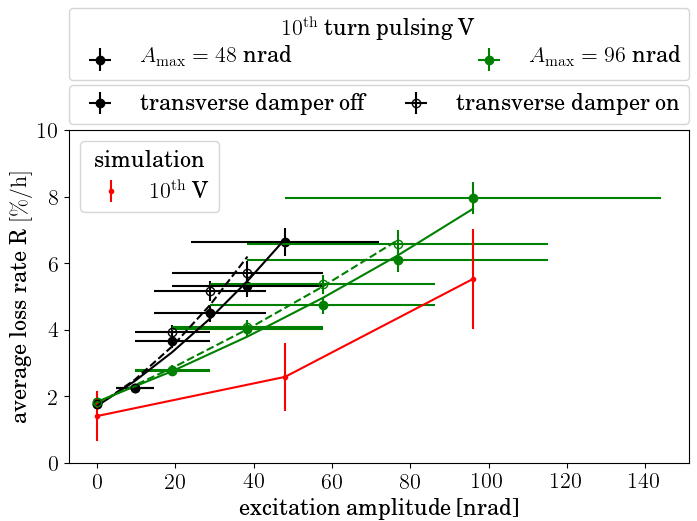
\includegraphics[width=1.0\linewidth]{2016_scale_amp_10v_ran_lblshort_sim_prstab.png}
	\caption{\label{fig:10thexploss} Comparison of scaling of loss rates $R$ as defined in Eqn.~\ref{eqn:lossrate} with the excitation amplitude for $10^{\mathrm{th}}$~turn pulsing in~V. The experimental results for a maximum excitation of $A_{\mathrm{max}}=48$~nrad are shown in black and for $A_{\mathrm{max}}=96$~nrad in green. The excitation amplitude error is 50\% and the error on the loss rate is the pure statistical error on the mean. The simulation results (see Fig.~\ref{fig:10thsim}) for 2016 injection optics, standard errors, $(Q_x,Q_y)=(64.28,59.31)$, $10^{\mathrm{th}}$~turn pulsing in V plus random dipole noise in H+V of 6~nrad are shown in red together with their statistical error. The loss rates follow approximately a quadratic behavior illustrated by a second order polynomial fit to the data shown as solid (for bunches with transverse damper off) or dashed (for bunches with transverse damper on) line.}
\end{figure}

\clearpage

\subsection{$7^{\mathrm{th}}$ turn pulsing\label{sec:simex7}}
The $7^{\mathrm{th}}$~turn pulsing pattern has been tested during both experiments in 2016 and 2017. In 2016 the resonant excitation was tested for the first time in the LHC and the experiments were therefore still in the exploratory state. Based on the experience gained in 2016, the experiments could then be repeated more systematically with more bunches allowing to also test in addition the dependence on the excitation plane. Also in case of the $7^{\mathrm{th}}$~turn pulsing, the experiment in 2016 as well as in 2017 can be divided in different parts: the first part without excitation, the second part with a resonant excitation with a maximum amplitude of $A_{\mathrm{max}}=6$~nrad, a third part in which the excitation amplitude is further increased to $A_{\mathrm{max}}=12$~nrad and in case of the 2016 experiments even further to $A_{\mathrm{max}}=24$~nrad. As the machine tune was changed in standard operation from (64.28,59.31) in 2016 to (62.27,60.295) in 2017 accompanied by a slight change in optics, considered irrelevant in the context of the presented measurements, a direct comparison of the two experiments and thus check of reproducibility is however not possible. 

The described change in tune entailed a change in the driving resonances, from previously the $7Q_x$ resonances in 2016 to mainly the $7Q_x$ and $7Q_y$ resonance in 2017. This can be seen from the FMA analysis for the 2016 optics (see Fig.~\ref{fig:patternfma} bottom left and bottom right), which shows a strong increase in diffusion for $7^{\mathrm{th}}$~turn pulsing in H around the $7Q_x$ resonances and only small changes for pulsing in V. In case of the 2017 optics and tune, the $7Q_x$ as well as the $7Q_y$ resonances cross the tune footprint (see Fig.~\ref{fig:7th2017fma} top left) and are also excited by the $7^{\mathrm{th}}$~turn pulsing visible as an increase of the diffusion in tune around the corresponding resonance lines for pulsing only in H or only in V and thus also for H+V (see Fig.~\ref{fig:7th2017fma}). An increase in the diffusion in tune however much weaker than for the $7Q_x$ and $7Q_y$ resonances is also observed around the $7Q_x + 7Q_y$ resonances for pulsing in V and H+V suggesting also an excitation of this $14^{\mathrm{th}}$ order resonance in addition. Why it is not visible for pulsing only in H is not understood.
\begin{figure*}[h]
	\begin{minipage}[t]{0.49\linewidth}
		\centering
		no excitation
		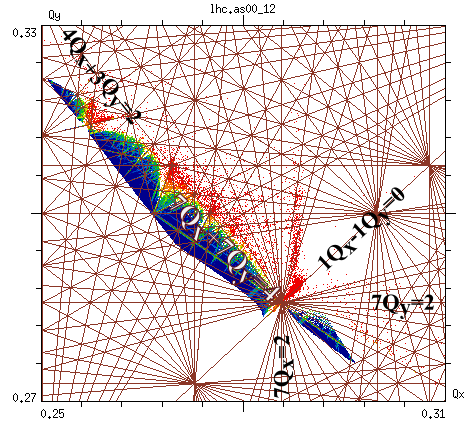
\includegraphics[width=1.0\linewidth]{2017injnocolc15o+19_6noerru_dp0_ord14_annotate_7th.png}
	\end{minipage}
	\begin{minipage}[t]{0.49\linewidth}
		\centering
		$7^{\mathrm{th}}$ H+V
		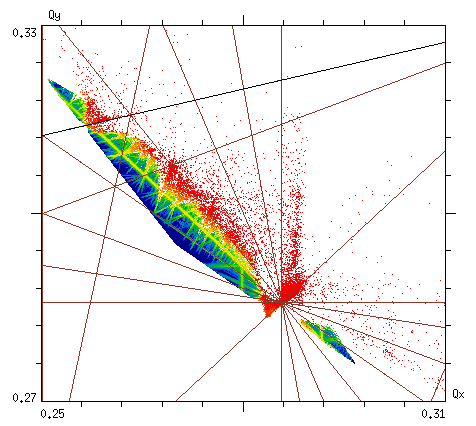
\includegraphics[width=1.0\linewidth]{2017injnocolc15o+19_6noerrut7skhv_dp0_ord7.png}
	\end{minipage}	
	\begin{minipage}[t]{0.49\linewidth}
		\centering
		$7^{\mathrm{th}}$ H
		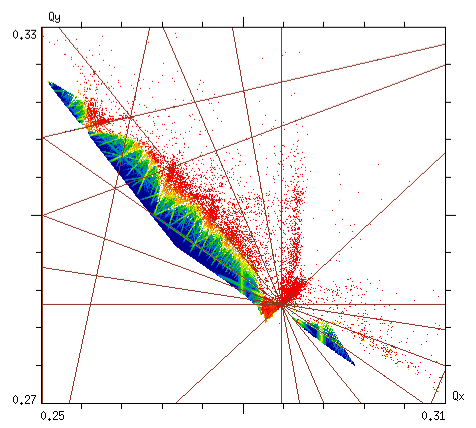
\includegraphics[width=1.0\linewidth]{2017injnocolc15o+19_6noerrut7skh_dp0_ord7.png}
	\end{minipage}
	\begin{minipage}[t]{0.49\linewidth}
		\centering
		$7^{\mathrm{th}}$ V
		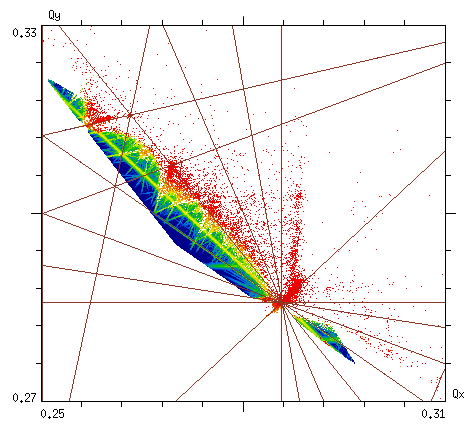
\includegraphics[width=1.0\linewidth]{2017injnocolc15o+19_6noerrut7skv_dp0_ord7.png}
	\end{minipage}	
	\caption{\label{fig:7th2017fma} FMA analysis in frequency space without excitation (top left) and for $7^{\mathrm{th}}$~turn pulsing in H+V (top right), only in H (bottom left) and only in V (bottom right) based on the 2017 injection optics with no machine errors and a tune of (62.27,60.295). The excitation is 96~nrad in both planes. The $7Q_x$ and $7Q_y$ resonance are both excited and in addition to the 14th order $7Q_x+7Q_y$.}
\end{figure*}

\begin{table}[b]
	\caption{\label{tab:7thexp}%
		Overview of the effect of $7^{\mathrm{th}}$~turn pulsing during the two resonant excitation experiments in 2016~\cite{resexmd2016} and 2017~\cite{resexmd2017}. The plane of the excitation is abbreviated with H for horizontal, V for vertical and H+V for horizontal and vertical at the same time.
	}
	\begin{ruledtabular}
		\begin{tabular}{lcc}
			Parameter & Experiment 2017 & Experiment 2016  \\
			\colrule
			optics & 2017 injection optics & 2016 injection optics \\
			tune $(Q_x,Q_y)$ & (62.27,60.295) & (64.28,59.31)\\\hline
			excitation plane  & H,V and H+V&  H\\
			losses & similar loss rates for  & large losses for \\
			& pulsing in H,V &  pulsing in H \\
			&  and H+V & \\
			hor. emit. growth & no & yes, very small \\
			vert. emit. growth & yes, for pulsing in & no\\
			&  V and H+V & \\
		\end{tabular}
	\end{ruledtabular}
\end{table}

\begin{figure*}[h]
	\begin{minipage}[t]{0.49\linewidth}
		\centering
		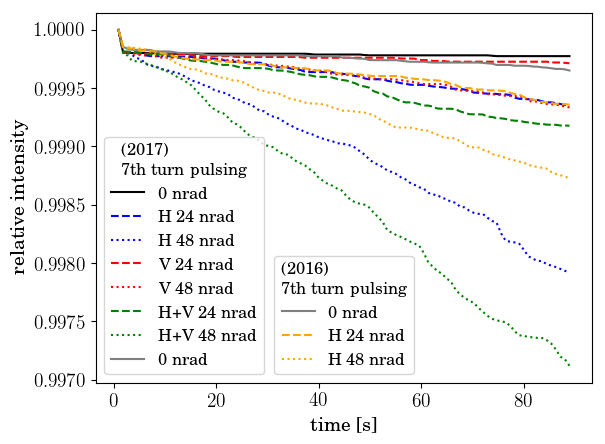
\includegraphics[width=1.0\linewidth]{2016+2017injerra2b2uran1_2e-3_7th_3_5um_intensity.png}
	\end{minipage}
	\begin{minipage}[t]{0.49\linewidth}
		\centering
		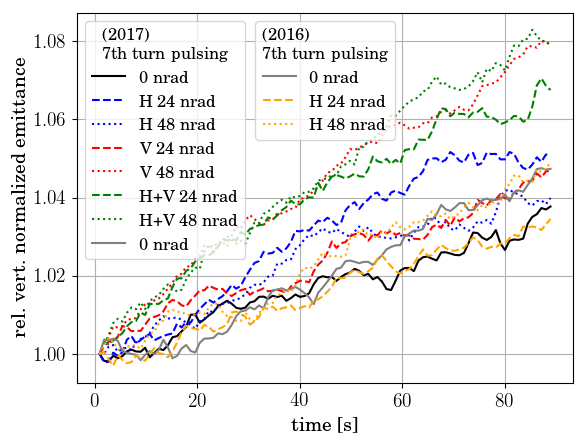
\includegraphics[width=1.0\linewidth]{2016+2017injerra2b2uran1_2e-3_7th_3_5um_rel_emit2.png}
	\end{minipage}
	\begin{minipage}[t]{0.49\linewidth}
		\centering
		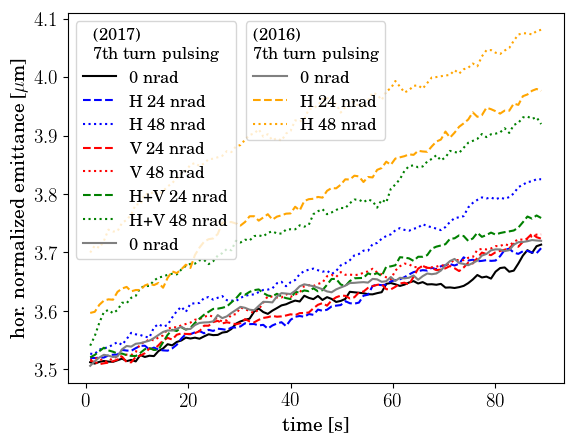
\includegraphics[width=1.0\linewidth]{2016+2017injerra2b2uran1_2e-3_7th_3_5um_emit1.png}
	\end{minipage}	
	\begin{minipage}[t]{0.49\linewidth}
		\centering
		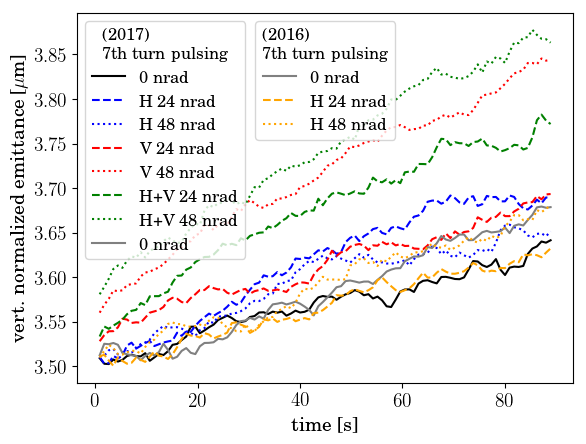
\includegraphics[width=1.0\linewidth]{2016+2017injerra2b2uran1_2e-3_7th_3_5um_emit2.png}
	\end{minipage}
	\caption{\label{fig:7thsim} Relative intensity (top left), relative vertical emittance (top right), and horizontal (bottom left) and vertical (bottom right) emittance obtained from distribution tracking based on the 2016 injection optics with standard errors and $(Q_x,Q_y)=(64.28,59.31)$ and 2017 injection optics with standard errors and $(Q_x,Q_y)=(62.27,60.295)$. The solid line indicates an excitation with only a random dipole noise component in H+V of 6~nrad, and the dotted and dashed line the results for $7^{\mathrm{th}}$~turn pulsing with two different excitation amplitudes plus a random dipole noise component in H+V of 6~nrad.}
\end{figure*}

The simulation results from the distribution tracking shown in Fig.~\ref{fig:7thsim} in general predict in terms of emittance for the two experiments:
\begin{description}
	\item[2016 experiment] Excitation amplitude dependent emittance growth in the horizontal but not in the vertical plane.
	\item[2017 experiment] Excitation amplitude dependent emittance growth in the vertical plane but not in the horizontal plane for an excitation in V and H+V. For an excitation only in H no emittance growth is observed.
\end{description}
Similar changes of the emittance as predicted in simulations were also experimentally observed as depicted in Fig.~\ref{fig:7thexp}, where emittance growth was observed only in the horizontal plane for pulsing in H in 2016, and only in the vertical plane for pulsing in V and H+V in 2017 with no emittance growth at all for pulsing in H. Just as for the $10^{\mathrm{th}}$~turn pulsing, the emittance growth can be divided also for the $7^{\mathrm{th}}$~turn pulsing in a phase of fast adjustment of the beam distribution and the reach of a new equilibrium state indicated in blue (fast adjustment) and black (equilibrium state) in Fig.~\ref{fig:7thexp}. Also in this case, the distribution changes are directly visible on the beam profiles taken with the BSRT (see Appendix~\ref{app:sec:7}, Fig.~\ref{fig:7thexpprof}).
\begin{figure*}[h]
		2016 experiment, $7^\mathrm{th}$ H	\\	\begin{minipage}[t]{0.32\linewidth}
		\centering
		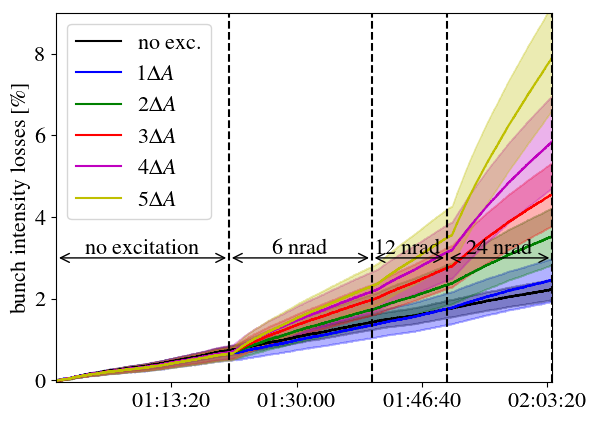
\includegraphics[height=0.75\linewidth]{2016_bunch_intensity_h7th_no_damper_avg.png}
	\end{minipage}	
	\begin{minipage}[t]{0.32\linewidth}
		\centering
		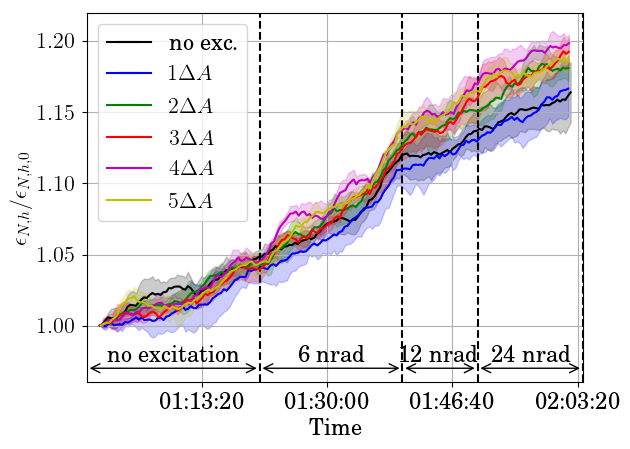
\includegraphics[height=0.75\linewidth]{2016_emith_avg_rel_h7th_no_damper.png}
	\end{minipage}	
	\begin{minipage}[t]{0.32\linewidth}
		\centering
		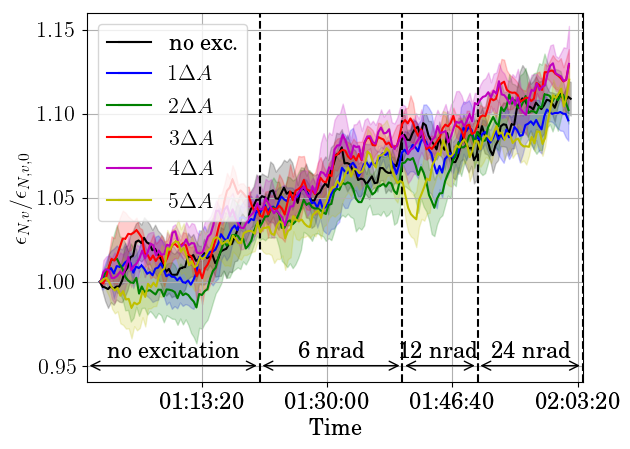
\includegraphics[height=0.75\linewidth]{2016_emitv_avg_rel_h7th_no_damper.png}
	\end{minipage}	
		2017 experiment, $7^\mathrm{th}$ H+V\\
	\begin{minipage}[t]{0.32\linewidth}
		\centering
		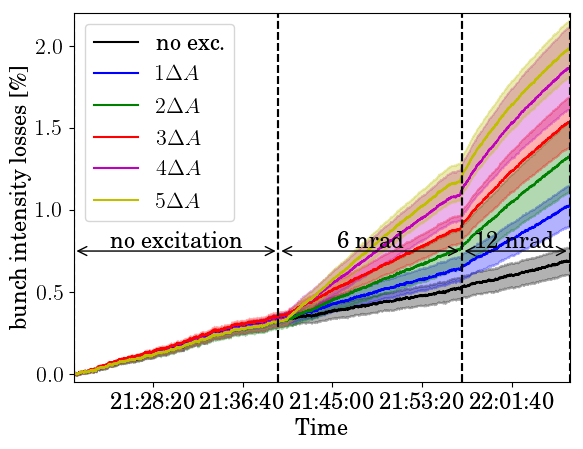
\includegraphics[height=0.75\linewidth]{2017_bunch_intensity_hv7th_no_damper_avg.png}
	\end{minipage}	
	\begin{minipage}[t]{0.32\linewidth}
		\centering
		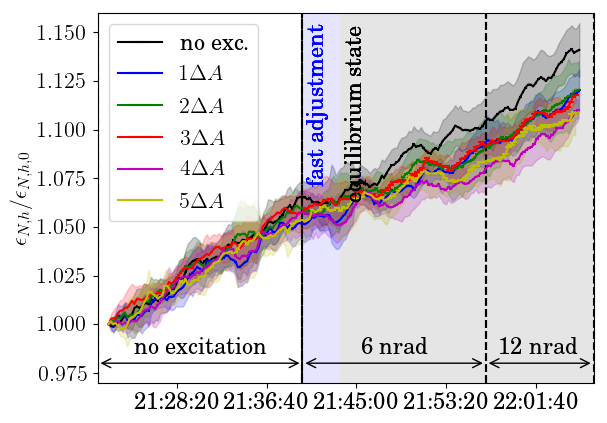
\includegraphics[height=0.75\linewidth]{2017_emith_avg_rel_hv7th_no_damper.png}
	\end{minipage}	
	\begin{minipage}[t]{0.32\linewidth}
		\centering
		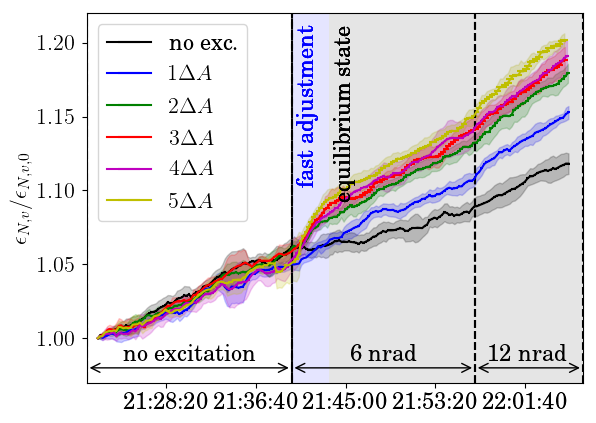
\includegraphics[height=0.75\linewidth]{2017_emitv_avg_rel_hv7th_no_damper.png}
	\end{minipage}	
	\caption{\label{fig:7thexp} Relative horizontal (top) and vertical (bottom) emittance obtained during the 2016 experiments (left) and the 2017 experiment (right) averaged over the bunches experiencing the same excitation amplitude. For all bunches the damper was not active.}
\end{figure*}

The losses measured during the experiment however differ from the simulations in terms of for which case the largest rate is observed as well as quantitatively for the specific cases. For example smaller losses are expected for the 2016 experiments compared to the 2017 experiments from simulations, while experimentally higher loss rates were measured in 2016 (see Fig.~\ref{fig:7thexploss}). For the 2017 experiment, the highest loss rates are expected for pulsing in H+V, than in H and then with a considerably reduction in V. During the experiment comparable loss rates are however measured for all three planes (see Appendix~\ref{app:sec:7}, Fig.~\ref{fig:7thexploss2017}). Last but not least the loss rates as defined in Eqn.~\ref{eqn:lossrate} for the 2016 (red and yellow) and 2017 (black and gree) experiments are compared in Fig.~\ref{fig:7thexploss}. In both cases and as also observed for the $10^{\mathrm{th}}$~turn pulsing, the loss rate follows a quadratic scaling with the excitation amplitude. Loss rates were in general higher during the 2016 experiments. The loss rates from simulations are not shown in Fig.~\ref{fig:7thexploss} as losses were only observed for much higher excitation amplitudes than tried in the experiments.
\begin{figure}[h]
	\centering
	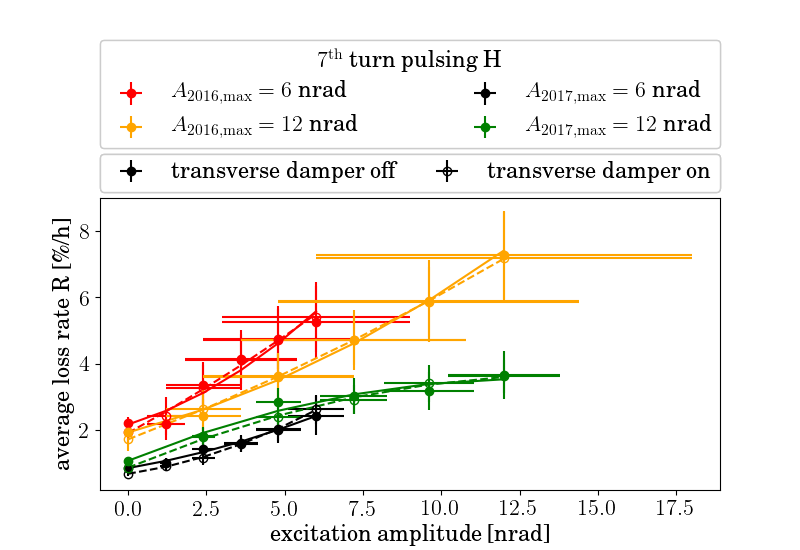
\includegraphics[width=1.0\linewidth]{2016+2017_scale_amp_7h_lblshort.png}
	\caption{\label{fig:7thexploss} Comparison of scaling of loss rates with excitation amplitude for $7^{\mathrm{th}}$~turn pulsing in H and data obtained during the 2016 experiment (black and blue) and 2017 experiment (red and yellow). The excitation amplitude error is 50\% in 2016 and was reduced to 15\% in 2017. The solid and dashed line indicate the second order polynomial fit to the loss rate.}
\end{figure}

\clearpage

\subsection{$8^{\mathrm{th}}$ turn pulsing\label{sec:simex8}}
Pulsing patterns which have little effect on the beam core are particularly interesting for the hollow electron lens operation if they in addition have a large effect on the halo. This is in general feasible considering the highly nonlinear field generated at the location of the halo particles by the HEL compared to no field or only a very small field at the location of the beam core. With this motivation in mind the $8^{\mathrm{th}}$~turn pulsing pattern was studied, for which a small effect in comparison to the $7^{\mathrm{th}}$ and $10^{\mathrm{th}}$ turn pulsing is expected (see Fig.~\ref{fig:8thsim}).
\begin{figure*}[h]
	\begin{minipage}[t]{0.49\linewidth}
		\centering
		\includegraphics[width=1.0\linewidth]{2017injerra2b2uran1_2e-3_8th_3_5um_intensity.png}
	\end{minipage}
	\begin{minipage}[t]{0.49\linewidth}
		\centering
		\includegraphics[width=1.0\linewidth]{2017injerra2b2uran1_2e-3_8th_3_5um_sigm.png}
	\end{minipage}
	\begin{minipage}[t]{0.49\linewidth}
		\centering
		\includegraphics[width=1.0\linewidth]{2017injerra2b2uran1_2e-3_8th_3_5um_emit1.png}
	\end{minipage}	
	\begin{minipage}[t]{0.49\linewidth}
		\centering
		\includegraphics[width=1.0\linewidth]{2017injerra2b2uran1_2e-3_8th_3_5um_emit2.png}
	\end{minipage}	
	\caption{\label{fig:8thsim} Relative intensity (top left), bunch length (top right), and horizontal (bottom left) and vertical (bottom right) emittance obtained from simulations (distribution tracking) based on the 2017 injection optics with standard errors and $(Q_x,Q_y)=(62.27,60.295)$. The solid line indicates an excitation with only a random dipole noise component in H+V of 6~nrad, and the dotted and dashed line the results for $8^{\mathrm{th}}$~turn pulsing plus a random dipole noise component in H+V of 6~nrad.}
\end{figure*}
\begin{figure*}[t]
	\begin{minipage}[t]{0.49\linewidth}
		\centering
		no excitation
		\includegraphics[width=1.0\linewidth]{2017injnocolc15o+19_6noerru_dp0_amp.png}
	\end{minipage}
	\begin{minipage}[t]{0.49\linewidth}
		\centering
		$8^{\mathrm{th}}$ H+V
		\includegraphics[width=1.0\linewidth]{2017injnocolc15o+19_6noerrut8skhv_dp0_amp_annotate.png}
	\end{minipage}	
	\caption{\label{fig:8th2017fmaamp} FMA analysis in amplitude space without excitation (left) and for $8^{\mathrm{th}}$~turn pulsing (right) based on the 2017 injection optics with no machine errors and a tune of (62.27,60.295). The excitation is 96~nrad in both planes. The $16Q_y$ and \mbox{$8Q_x-4Q_y$} are both excited.}
\end{figure*}
In simulations no visible effect is indeed observed for excitation amplitudes smaller than 96~nrad. In the horizontal and vertical plane a small emittance growth due to the excitation is visible, but without any clear dependence on the amplitude or plane. The FMA analysis in amplitude space reveals also the driven resonances (Fig.~\ref{fig:8th2017fmaamp}), which are the $16Q_y$ and \mbox{$8Q_x-4Q_y$} resonances and several even higher orders. These are in general very high order resonances whose effect is thus expected to be small.

\begin{figure}[h]
	\centering
	\includegraphics[width=1.0\linewidth]{2017_scale_amp_8hv_lblshort.png}
	\caption{\label{fig:8thexploss} Comparison of scaling of loss rates with excitation amplitude for $8^{\mathrm{th}}$~turn pulsing in H+V measured during the 2017 experiment. The excitation amplitude error is 15\% indicated by the horizontal error bars, the error on the loss rate is the error on the mean obtained through the average over the 6~bunches with the same excitation amplitude.}
\end{figure}
The small effect on the beam expected from simulations could then be also confirmed experimentally during the 2017 experiment. For this purpose the excitation amplitude was increased to the maximum reachable amplitude of 96~nrad. As depicted in Fig.~\ref{fig:8thexploss}, the loss rate increased slightly with the excitation amplitude for an excitation in H+V. For an excitation only in V or only in H, no statistically relevant increase was observed (see Appendix~\ref{app:sec:8}, Fig.~\ref{fig:8thexploss2017}). In the horizontal plane, a change in beam distribution was measured with the BSRT profiles (Appendix~\ref{app:sec:8}, Fig.~\ref{fig:8thexpprof}) for an excitation only in~H. The distribution increased around $2.0~\sigma$ simultaneously with a depletion of the beam core. For an excitation in H+V one would expect to see a similar distribution change. However, this change is not visible as the emittance of the references bunches was much smaller, around $1.8~\mu$m normalized emittance, compared to around $2.6~\mu$m for the excited bunches \cite{resexmd2017}. This difference in emittance then resulted in a stronger emittance growth due to intra-beam scattering for the reference bunches in comparison to the excited bunches making the additional emittance growth and distribution changes due to the excitation undetectable. In the vertical plane, the beam distribution and emittance were not affected by the resonant excitation.

\clearpage

\subsection{random excitation\label{sec:simexran}}
The random excitation presents in general the pulsing pattern leading to the fastest halo depletion rates achievable with an HEL. On the other hand this pattern is also the most dangerous one for the proton beam core. The aim of this experiment was to test the effect on the core in comparison to the resonant excitation represented in the 2017 experiment by primarily the $7^{\mathrm{th}}$~turn pulsing as for $8^{\mathrm{th}}$~turn pulsing basically no effect was observed. The random excitation is in general so powerful as it excites all frequencies of the beam equally.
\begin{figure*}[h]
	\begin{minipage}[t]{0.49\linewidth}
		\centering
		no excitation
		\includegraphics[width=1.0\linewidth]{2017injnocolc15o+19_6noerru_dp0_amp.png}
	\end{minipage}
	\begin{minipage}[t]{0.49\linewidth}
		\centering
		uniform random H+V
		\includegraphics[width=1.0\linewidth]{2017injnocolc15o+19_6noerruranadthv_1nrad_dp0_amp.png}
	\end{minipage}	
	\caption{\label{fig:ran2017fmaamp} FMA analysis in amplitude space without excitation (left) and for a uniform random excitation with 1~nrad amplitude (right) in H+V based on the 2017 injection optics with no machine errors and a tune of (62.27,60.295).}
\end{figure*}
This can be seen clearly on the example of the FMA analysis in amplitude space depicted in Fig.~\ref{fig:ran2017fmaamp}. In the case of a random excitation, the diffusion in tune is increased in comparison to the $k^{\mathrm{th}}$~turn pulsing rather equally for all particle amplitudes.
\begin{figure*}[h]
	\begin{minipage}[t]{0.49\linewidth}
		\centering
		\includegraphics[width=1.0\linewidth]{2017injerra2b2u_ranadt_3_5um_intensity.png}
	\end{minipage}
	\begin{minipage}[t]{0.49\linewidth}
		\centering
		\includegraphics[width=1.0\linewidth]{2017injerra2b2u_ranadt_3_5um_sigm.png}
	\end{minipage}
	\begin{minipage}[t]{0.49\linewidth}
		\centering
		\includegraphics[width=1.0\linewidth]{2017injerra2b2u_ranadt_3_5um_emit1.png}
	\end{minipage}	
	\begin{minipage}[t]{0.49\linewidth}
		\centering
		\includegraphics[width=1.0\linewidth]{2017injerra2b2u_ranadt_3_5um_emit2.png}
	\end{minipage}
	\caption{\label{fig:ransim} Relative intensity (top left), bunch length (top right), and horizontal (bottom left) and vertical (bottom right) emittance obtained from distribution tracking based on the 2017 injection optics with standard errors and $(Q_x,Q_y)=(62.27,60.295)$. The solid line indicates the case with no excitation, and the dotted and dashed line the results for a uniform random excitation of 12~nrad and 24~nrad respectively.}
\end{figure*}
The distribution tracking shown in Fig.~\ref{fig:ransim} also reveals a quite symmetric evolution of the beam parameters for a random excitation:
\begin{itemize}
	\item Emittance growth is only caused by an excitation in the same plane.
	\item The emittance growth is quantitatively comparable for an excitation in only the corresponding plane. Only a small increase or decrease is observed if the excitation is applied in both planes. The difference could be due to coupling.
	\item The random excitation leads to an increase of the emittance growth rate. Compared to the $k^{\mathrm{th}}$~turn pulsing there is explicitly no initial adjustment phase of the distribution.
	\item Negligible losses are observed independent of the plane of excitation.
\end{itemize}
\begin{figure*}[b]
	random excitation V\\
	\begin{minipage}[t]{0.32\linewidth}
		\centering
		\includegraphics[height=0.75\linewidth]{2017_bunch_intensity_vran_no_damper_avg.png}
	\end{minipage}	
	\begin{minipage}[t]{0.32\linewidth}
		\centering
		\includegraphics[height=0.75\linewidth]{2017_emith_avg_rel_vran_no_damper.png}
	\end{minipage}	
	\begin{minipage}[t]{0.32\linewidth}
		\centering
		\includegraphics[height=0.75\linewidth]{2017_emitv_avg_rel_vran_no_damper.png}
	\end{minipage}	
		random excitation H+V\\
	\begin{minipage}[t]{0.32\linewidth}
		\centering
		\includegraphics[height=0.75\linewidth]{2017_bunch_intensity_hvran_no_damper_avg.png}
	\end{minipage}	
	\begin{minipage}[t]{0.32\linewidth}
		\centering
		\includegraphics[height=0.75\linewidth]{2017_emith_avg_rel_hvran_no_damper.png}
	\end{minipage}	
	\begin{minipage}[t]{0.32\linewidth}
		\centering
		\includegraphics[height=0.75\linewidth]{2017_emitv_avg_rel_hvran_no_damper.png}
	\end{minipage}	
	\caption{\label{fig:ranexp} Relative intensity (left) and relative horizontal (center) and vertical (right) emittance for a random excitation only in V (top) and in H+V (bottom). Emittance growth is only caused in the plane of excitation.}
\end{figure*}

Qualitatively, this behavior could be also confirmed experimentally during the 2017 experiments. Here excitation amplitude dependent emittance growth was only recorded in the plane of excitation with all excitation amplitude dependent emittance growth rates in a comparable range. As example the relative horizontal and vertical emittance for pulsing in V and in H+V are depicted in Fig.~\ref{fig:ranexp}. Note that as expected from simulations and despite the large excitation amplitude dependent emittance growth, the growth rates stays constant. There is explicitly no fast adjustment phase succeeded by a new equilibrium state as observed for the $7^{\mathrm{th}}$ and $10^{\mathrm{th}}$~turn pulsing.
\begin{figure*}[h]
	\begin{minipage}[t]{0.49\linewidth}
		\centering
		reference bunch,\\ no excitation
		\includegraphics[width=1.0\linewidth]{profile_v_ranv_slot_1698.png}
	\end{minipage}
	\begin{minipage}[t]{0.49\linewidth}
		\centering
		excited bunch,\\ random excitation V
		\includegraphics[width=1.0\linewidth]{profile_v_ranv_slot_1532.png}
	\end{minipage}
	\caption{\label{fig:ranexpprof}Vertical beam profiles measured with the Beam Synchrotron Radiation Telescope (BSRT) during the 2017 experiments. The profiles are taken at the end of the random excitation in V. For both bunches the transverse damper is not active. The distribution changes in the reference bunch (left), here slot 1698, are much less than for the bunch experiencing the maximum excitation (right), here slot 2696.}
\end{figure*}
The changes in emittance are also directly visible in the beam profiles measured with the BSRT. As an example Fig.~\ref{fig:ranexpprof} shows the profile for a random excitation only in V in comparison to a reference bunch. The distribution also stays Gaussian in case of a random excitation in contrast to the $10^{\mathrm{th}}$~turn pulsing in which case it clearly assumes a non-Gaussian shape (see Fig.~\ref{fig:10thexpprof}).

\begin{figure*}[h]
	\begin{minipage}[t]{0.32\linewidth}
		\centering
		\includegraphics[width=1.0\linewidth]{2017_scale_amp_ranh_lblshort.png}
	\end{minipage}	
	\begin{minipage}[t]{0.32\linewidth}
		\centering
		\includegraphics[width=1.0\linewidth]{2017_scale_amp_ranv_lblshort.png}
	\end{minipage}	
	\begin{minipage}[t]{0.32\linewidth}
		\centering
		\includegraphics[width=1.0\linewidth]{2017_scale_amp_ranhv_lblshort.png}
	\end{minipage}	
	\caption{\label{fig:ranexplossplane} Comparison of scaling of loss rates with excitation amplitude for a random excitation only in H (top), only in V (center) and in H+V (bottom) measured during the 2017 experiment. The excitation amplitude error is 15\% indicated by the horizontal error bars. The loss rate is considerably reduced for the bunches with transverse damper active and is approximately additive with the excitation plane, meaning that double the loss rate is observed for an excitation in H+V compared to only in H or only in V.}
\end{figure*}
The experimental results for a maximum excitation amplitude of $A_{\mathrm{max}}=1$~nrad and $A_{\mathrm{max}}=6$~nrad also confirm the in general small losses predicted in simulations. The losses then increase more dramatically around the time when the maximum excitation amplitude is increased to $A_{\mathrm{max}}=12$~nrad (see Fig.~\ref{fig:ranexpprof}). This is most likely the point when, due to the large emittance growth, the physical aperture starts cutting into the more central region of the distribution. Furthermore, the dependence of the loss rate on the excitation plane is additive, meaning that double the loss rate is observed for an excitation in H+V compared to only in H or only V. The loss rate is also considerably reduced for the bunches with transverse damper active independent of the plane the excitation is applied in (see Fig.~\ref{fig:ranexplossplane}). In comparison to the $7^{\mathrm{th}}$~turn pulsing, the loss rate for a random excitation is smaller for a maximum excitation amplitude of $A_{\mathrm{max}}=6$~nrad, but larger for $A_{\mathrm{max}}=12$~nrad (see Fig.~\ref{fig:ranexploss}). This indicates an increase of the diffusion mostly in the beam tails for $7^{\mathrm{th}}$~turn pulsing, while for a random excitation mostly the core is affected.
\begin{figure}[h]
	\centering
	\includegraphics[width=1.0\linewidth]{2017_scale_amp_7th_ranhv_lblshort.png}
	\caption{\label{fig:ranexploss}  Comparison of scaling of loss rates with excitation amplitude for a random excitation and $7^{\mathrm{th}}$~turn pulsing in H+V measured during the 2017 experiment. The excitation amplitude error is 15\% indicated by the horizontal error bars.}
\end{figure}

\clearpage

\subsection{Effect of the transverse damper\label{sec:damp}}
\begin{figure*}[b]
	\centering
	damper not active\\
	\begin{minipage}[t]{0.32\linewidth}
		\centering
	random excitation V, 2017\\
		\includegraphics[height=0.75\linewidth]{2017_emitv_avg_rel_vran_no_damper.png}
	\end{minipage}	
	\begin{minipage}[t]{0.32\linewidth}
		\centering
		$7^{\mathrm{th}}$~turn V, 2017 exp.\\
		\includegraphics[height=0.75\linewidth]{2017_emitv_avg_rel_v7th_no_damper_no_text.png}
	\end{minipage}	
	\begin{minipage}[t]{0.32\linewidth}
		\centering
		$10^{\mathrm{th}}$~turn V, 2016 exp.\\
		\includegraphics[height=0.75\linewidth]{2016_emitv_avg_rel_v10th_no_damper_no_text.png}
	\end{minipage}	
	damper active\\
	\begin{minipage}[t]{0.32\linewidth}
		\centering
		random excitation V, 2017 exp.\\
		\includegraphics[height=0.75\linewidth]{2017_emitv_avg_rel_vran_with_damper.png}
	\end{minipage}	
	\begin{minipage}[t]{0.32\linewidth}
		\centering
		$7^{\mathrm{th}}$~turn V, 2017 exp.\\
		\includegraphics[height=0.75\linewidth]{2017_emitv_avg_rel_v7th_with_damper_no_text.png}
	\end{minipage}	
	\begin{minipage}[t]{0.32\linewidth}
		\centering
		$10^{\mathrm{th}}$~turn V, 2016 exp.\\
		\includegraphics[height=0.75\linewidth]{2016_emitv_avg_rel_v10th_with_damper_no_text.png}
	\end{minipage}	
	\caption{\label{fig:damp} Relative intensity for bunches with transverse damper not active (top) and transverse damper active (bottom) for a random excitation only in V (left) and for $7^{\mathrm{th}}$ (center) and $10^{\mathrm{th}}$~turn pulsing only in V (right).}
\end{figure*}
For all $k^{\mathrm{th}}$~turn pulsing patterns tested experimentally, the transverse damper does in general not change any of the observables studied during the experiments, explicitly losses, emittance and beam distribution suggesting that indeed it is not damping any resonant excitation. On the other hand, the transverse damper considerably decreases any changes of the above parameters in case of a random excitation. As an example, the vertical emittance growth for the $7^{\mathrm{th}}$ and $10^{\mathrm{th}}$~turn pulsing in V is compared with a random excitation in V in Fig.~\ref{fig:damp}. The same observation is also made in case of losses as shown in Fig.~\ref{fig:ranexploss} comparing the $7^{\mathrm{th}}$~turn pulsing in H+V with a random excitation in H+V. For the $7^{\mathrm{th}}$~turn pulsing the two curves for the transverse damper active and not active almost coincide while for the random excitation a significant difference is visible. Until present, it is unknown why the transverse damper (ADT) appears to be incapable of damping any resonant excitation as it fulfills all requirements to detect as well as damp the caused oscillation:
\begin{itemize}
	\item The closed orbit distortion caused by the resonant excitation during the experiments is large enough to be detectable with the ADT pickups.
	\item The ADT compares the position of each bunch with its position in the previous turn in order to detect an orbit distortion to be damped. Therefore an oscillation due to any $k^{\mathrm{th}}$~turn pulsing with $k>1$ would be noticed and damped.
	\item The ADT is capable of damping the oscillation of each bunch individually. The ADT should therefore be capable of applying the correct corrective kick for each group of bunches seeing the same excitation amplitude.
\end{itemize}
Further studies are therefore needed in order to obtain a deeper understanding of the interaction of the transverse damper with a resonant excitation.
\clearpage

\section{Summary\label{sec:sum}}
This paper intends to give an overview of the effects of the hollow electron lens (HEL) on the proton beam core and the experiments conducted in this context at the LHC in 2016~\cite{resexmd2016} and 2017~\cite{resexmd2017}. For a perfect HEL without any imperfections no effect on the core is to be expected as the field at the center vanishes by construction. Only in the case of imperfections in the guidance and profile of the electron beam, a residual kick on the proton beam core can occur. In this case and assuming HL-LHC parameters (Tables~\ref{tab:hllhc_param}--\ref{tab:hel_param}), the contribution from the electron lens bends with approximately $0.5$~nrad to first order is negligible with respect to the kick expected from the central region of the HEL of approximatley $20$~nrad to first order caused by profile imperfections in the electron beam. In DC operation these kicks, even if nonlinear in reality, are negligible compared to the nonlinearities present in the LHC and HL-LHC and are thus of no concern. The picture changes if the HEL is operated in pulsed mode, in which case noise is introduced on the halo particles (intended) as well as on the beam core (unintended) in the presence of imperfections of the HEL entailing much more stringent tolerances.

To study the effect on the beam core in case of the much more dangerous pulsed operation, beam experiments were conducted in 2016 and 2017 at injection. As no hollow electron lens is currently installed in the LHC, the in reality non-linear kick was emulated to first order by a dipole kick with the corresponding excitation pattern. The experimental results in general suggest that for the kick amplitudes as expected from the HEL, considerable effects are to be expected for a random excitation and certain resonant excitations, explicitly $7^{\mathrm{th}}$ and $10^{\mathrm{th}}$~turn pulsing during the conducted experiments. In addition, also one resonant excitation pattern, the $8^{\mathrm{th}}$~turn pulsing, was tested featuring a small effect on the beam core. Assuming that this pattern has a large effect on the beam halo, it would be an optimal candidate for a feasible HEL excitation pattern.

The resonant excitation in general features a rich nonlinear dynamics leading to a diversity in beam distribution and diffusion changes as can be seen for example from the very diverse effects of the different $k^{\mathrm{th}}$~turn pulsing patterns observed in simulations and experiments. The origin of this diversity is due to the fact that only certain frequencies and thus resonances are excited. Typical for the resonant excitation is also the fast adjustment of the beam distribution to a new equilibrium state which could be for the first time measured in the experiments and predicted in the simulations presented in this paper. The random excitation on the other hand excites all beam frequencies equally, leading to the highest increase in halo removal rates for the HEL \cite{hel_halo_hllhc_fitterer} but also the strongest effects on the core, mainly in terms of strong emittance growth as predicted in simulations, experiments and also a multitude of earlier publications on the subject of random noise. From the experiments the tolerances summarized in Table~\ref{tab:tolexp} could be obtained, where for each excitation pattern and plane the smallest kick amplitude is listed for which an increase in emittance or losses was observed.
\begin{table}
	\caption{\label{tab:tolexp}%
		Minimum kick amplitudes $\Delta z'$ for which either an increase in emittance or losses was observed during the LHC experiments. The tolerances are given for the case of the transverse damper not active. The same tolerances are obtained for the case with the damper active in case of all resonant excitation. In case of a random excitation the tolerance can be increased by roughly a factor~2.
	}
	\begin{ruledtabular}
		\begin{tabular}{lccc}
		pulsing pattern & exp. year & plane & $\Delta z' \ [\mathrm{nrad}]$  \\
			\colrule
			random & 2017 & H or V & 2.4 \\
			 & & H+V & 1.2 \\\hline
			$7^{\mathrm{th}}$~turn & 2016 & H & 2.4 \\
			 & 2017 & H & 2.4 \\
			 & 2017 & V & 1.2 \\
			 & 2017 & H+V & 1.2 \\\hline
			$8^{\mathrm{th}}$~turn & 2017 & H & 14.4 \\
			& 2017 & V & $>96$ \\
			& 2017 & H+V & 12 \\\hline
			$10^{\mathrm{th}}$~turn & 2016 & V & 9.6 \\
		\end{tabular}
	\end{ruledtabular}
\end{table}
Tolerances in case of a random excitation are extremely stringent. For a resonant excitation the effect depends strongly on the order $k$ of the $k^{\mathrm{th}}$~turn pulsing. For a future HEL, the pattern could therefore be tuned to the machine and beam configuration in order to yield a strong effect on the halo particles and small effect on the beam core. Compared to the estimated kick amplitude of the HEL on the beam core of
\begin{equation}
\Delta x', \Delta y' = 20 \ \mathrm{nrad}
\end{equation}
the tolerances for all experimentally tried pulsing pattern except for $8^{\mathrm{th}}$~turn pulsing in V lie below this value. As a next step, the experiment should be conducted at collision energy where the HEL is most needed. At collision energy the inherent noise level of the LHC is smaller which could lead to more relaxed tolerances than the ones obtained at injection energy.



\begin{acknowledgments}
We wish to acknowledge Giulia Papotti with her help with the preparations for the 2016 experiments and her general support from the operations side, Roderik Bruce and Gianluca Valentino for there very helpful suggestions in preparing the experiment at the LHC and we would like to thank all participants of the experiment for helping acquire the data presented in this paper. We wish to thank Sergei Nagaitsev for the very useful discussion and profound question to find out why the transverse damper is not damping any resonant excitation. We would like to acknowledge Dmitry Shatilov for his help with the Lifetrac code, and St\'{e}phane Fartoukh, Riccardo De Maria and Rogelio Tomás for their help with generating the appropiate optics model. We are grateful also for the support from the beam instrumentation team, in particular Enrico Bravin and Georges Trad, with the BSRT and are thankful for the collaboration with St\'{e}phania Papadopoulou and Fanouria Antonio for the analysis of the BSRT profiles.
\end{acknowledgments}

\newpage

\appendix
\section{Additional plots for 10th turn pulsing during the 2016 experiments}
\label{app:sec:10}
\begin{figure}[h]
	\begin{minipage}[t]{0.49\linewidth}
		\centering
		no excitation
		\includegraphics[width=1.0\linewidth]{2016injnocolc15o+19_6noerru_dp0_ord10_annotate.png}
	\end{minipage}
	\begin{minipage}[t]{0.49\linewidth}
		\centering
		$10^{\mathrm{th}}$ H+V
		\includegraphics[width=1.0\linewidth]{2016injnocolc15o+19_6noerrut10skhv_dp0_ord10.png}
	\end{minipage}	
	\begin{minipage}[t]{0.49\linewidth}
		\centering
		$10^{\mathrm{th}}$ H
		\includegraphics[width=1.0\linewidth]{2016injnocolc15o+19_6noerrut10skh_dp0_ord10.png}
	\end{minipage}	
	\begin{minipage}[t]{0.49\linewidth}
		\centering
		$10^{\mathrm{th}}$ V
		\includegraphics[width=1.0\linewidth]{2016injnocolc15o+19_6noerrut10skv_dp0_ord10.png}
	\end{minipage}
	\caption{\label{app:fig:fma:10} FMA analysis for $10^{\mathrm{th}}$~turn pulsing based on the 2016 injection optics with no machine errors and a tune of (64.28,59.31). The excitation is 120~nrad in the corresponding plane. There is no significant difference in the FMA analysis between pulsing only in H, only in V or in H+V.}
\end{figure}

\newpage

\section{Additional plots for $7^{\mathrm{th}}$~turn pulsing during 2017 experiments}
\label{app:sec:7}
\begin{figure}[h]
	\begin{minipage}[t]{1.0\linewidth}
	\centering
	\includegraphics[width=0.9\linewidth]{2017_scale_amp_7h_lblshort.png}
	\end{minipage}
	\begin{minipage}[t]{1.0\linewidth}
		\centering
		\includegraphics[width=0.9\linewidth]{2017_scale_amp_7v_lblshort.png}
	\end{minipage}
	\begin{minipage}[t]{1.0\linewidth}
		\centering
		\includegraphics[width=0.9\linewidth]{2017_scale_amp_7hv_lblshort.png}
	\end{minipage}
	\caption{\label{fig:7thexploss2017} Comparison of scaling of loss rates with excitation amplitude for $7^{\mathrm{th}}$~turn pulsing only in H (top), only in V (center) and in H+V (bottom) during the 2017 experiment. The excitation amplitude error is 15\% indicated by horizontal error bars. The vertical errorbars represent the pure statistical error based on the averaging over several bunches with the same excitation amplitude.}
\end{figure}
\begin{figure}[h]
	\begin{minipage}[t]{0.49\linewidth}
		\centering
		reference bunch,\\ no excitation
		\includegraphics[width=1.0\linewidth]{profile_v_7thhv_slot_2862.png}
	\end{minipage}
	\begin{minipage}[t]{0.49\linewidth}
		\centering
		excited bunch,\\ $7^{\mathrm{th}}$~turn H+V	
		\includegraphics[width=1.0\linewidth]{profile_v_7thhv_slot_2696.png}
	\end{minipage}
	\caption{\label{fig:7thexpprof} Vertical beam profiles measured with the Beam Synchrotron Radiation Telescope (BSRT) during the 2017 experiments. The profiles are taken at the end of the $7^{\mathrm{th}}$~turn pulsing in H+V. For both bunches the transverse damper is not active. The distribution changes in the reference bunch (left), here slot 2862, are much less than for the bunch experiencing the maximum excitation (right), here slot 2696.}
\end{figure}

\newpage

\section{Additional plots for $8^{\mathrm{th}}$~turn pulsing during 2017 experiments}
\label{app:sec:8}
\begin{figure}[h]
	\begin{minipage}[t]{1.0\linewidth}
		\centering
		\includegraphics[width=0.9\linewidth]{2017_scale_amp_8h_lblshort.png}
	\end{minipage}
	\begin{minipage}[t]{1.0\linewidth}
		\centering
		\includegraphics[width=0.9\linewidth]{2017_scale_amp_8v_lblshort.png}
	\end{minipage}
	\begin{minipage}[t]{1.0\linewidth}
		\centering
		\includegraphics[width=0.9\linewidth]{2017_scale_amp_8hv_lblshort.png}
	\end{minipage}
	\caption{\label{fig:8thexploss2017} Comparison of scaling of loss rates with excitation amplitude for $8^{\mathrm{th}}$~turn pulsing only in H (top), only in V (center) and in H+V (bottom) during the 2017 experiment. The excitation amplitude error is 15\% indicated by horizontal error bars. The vertical errorbars represent the pure statistical error based on the averaging over several bunches with the same excitation amplitude.}
\end{figure}
\begin{figure}[h]
	\begin{minipage}[t]{0.49\linewidth}
		\centering
		reference bunch,\\ no excitation
		\includegraphics[width=1.0\linewidth]{profile_h_8thh_slot_804.png}
	\end{minipage}
	\begin{minipage}[t]{0.49\linewidth}
		\centering
		excited bunch,\\ $8^{\mathrm{th}}$~turn H
		\includegraphics[width=1.0\linewidth]{profile_h_8thh_slot_632.png}
	\end{minipage}
	\caption{\label{fig:8thexpprof} Horizontal beam profiles measured with the Beam Synchrotron Radiation Telescope (BSRT) during the 2017 experiments. The profiles are taken at the end of the $8^{\mathrm{th}}$~turn pulsing in H. For both bunches the transverse damper is not active. The distribution changes in the reference bunch (left), here slot 804, are much less than for the bunch experiencing the maximum excitation (right), here slot 632.}
\end{figure}

\newpage

%\section{Additional plots for random excitation during 2017 experiments}
%\label{app:sec:ran}

\clearpage

\bibliography{bibliography}% Produces the bibliography via BibTeX.

\end{document}
%
% ****** End of file apssamp.tex ******
